\section{Getting started}\label{sec:start}\index{PISM!getting started}

This introduction is intended to be interactive and participatory, and it should work on \emph{your personal machine} as well as on a supercomputer.  Please try the commands and view the resulting files.  Do the runs with your own values for the options.  We can't hide the fact that PISM has lots of ``control knobs,'' but fiddling with them will help you get going.  Give it a try!

To install PISM see the \emph{Getting PISM} tab at \href{http://www.pism-docs.org}{\texttt{www.pism-docs.org}}.  Or get the PISM Installation Manual (PDF) at \url{http://www.pism-docs.org/wiki/lib/exe/fetch.php?media=pism_installation.pdf}.  Once PISM is installed, the executable \texttt{pismr} should be available on your system's ``path''; confirm this with ``\texttt{which pismr}''.  The instructions below assume you are using a \texttt{bash} shell or one that accepts \texttt{bash} syntax.  They also assume you have the PISM source code in the directory ``\texttt{pism/}''.

\subsection{A Greenland ice sheet example}

We get started with an extended example showing how to generate initial states for prognostic model experiments on the Greenland ice sheet.  Ice sheet and glacier model studies often involve modeling present and past states using actions like the ones demonstrated here.  Our particular choices made here are motivated by the evaluation of initialization methods in \cite{AschwandenAdalgeirsdottirKhroulev}.

We use data assembled by the \href{http://websrv.cs.umt.edu/isis/index.php/SeaRISE_Assessment}{Sea-level Response to Ice Sheet Evolution (SeaRISE)} assessment process\index{SeaRISE!data} \cite{Bindschadler2013SeaRISE}.  SeaRISE is a community-organized assessment process providing an upper bound on ice sheet contributions to sea level in the next 100--200 years, especially for the IPCC AR5 report in 2013.

This example is a hands-on first look at PISM.  It is not an in-depth tutorial, and some details of what is happening are only explained later in this Manual, which thoroughly discusses PISM options, nontrivial modeling choices, and how to preprocess input data.

The basic runs here, mostly on coarse $20$ and $10\,\textrm{km}$ grids, can be done on a typical workstation or laptop.  PISM is, however, designed to make high resolution (e.g.~$5\,\textrm{km}$ to $\sim500\,\textrm{m}$ grids for whole-Greenland ice sheet modeling) possible by exploiting large-scale parallel processing.  See \cite{AschwandenAdalgeirsdottirKhroulev,Golledgeetal2012,Golledgeetal2013}, among other published high-resolution PISM examples.


\subsection{Input data}

The NetCDF data used to initialize SeaRISE runs is freely-available online: 
\medskip

\centerline{\protect{\textbf{\url{http://websrv.cs.umt.edu/isis/index.php/Present_Day_Greenland}}}}
\medskip

\noindent To download the specific file we want, namely \texttt{Greenland_5km_v1.1.nc}, and preprocess it for PISM, do:
\begin{verbatim}
$ cd pism/examples/std-greenland
$ ./preprocess.sh
\end{verbatim}
\noindent The script \texttt{preprocess.sh} requires \texttt{wget} and also the NetCDF Operators (``NCO''; \url{http://nco.sourceforge.net/}).  It downloads the version 1.1 of the SeaRISE ``master'' present-day data set, which contains ice thickness and bedrock topography from BEDMAP \cite{BamberLayberryGogenini}, and modeled precipitation and surface mass balance rates from RACMO \cite{Ettemaetal2009}, among other fields.

In particular, it creates three new NetCDF files which can be read by PISM.  The spatially-varying fields, with adjusted metadata, go in \texttt{pism_Greenland_5km_v1.1.nc}.  The other two new files contain famous time-dependent paleo-climate records from ice and seabed cores: \texttt{pism_dT.nc} has the GRIP temperature record \cite{JohnsenetalGRIP} and \texttt{pism_dSL.nc} has the SPECMAP sea level record \cite{Imbrieetal1984}.

Any of these NetCDF files can be viewed with \texttt{ncview} or other NetCDF visualization tools; see Table \ref{tab:NetCDFview} below.  An application of IDV to the master data set produced Figure \ref{fig:sr-input}, for example.  Use \texttt{ncdump -h} to see the metadata and history of the files.

\begin{figure}[ht]
\centering
\mbox{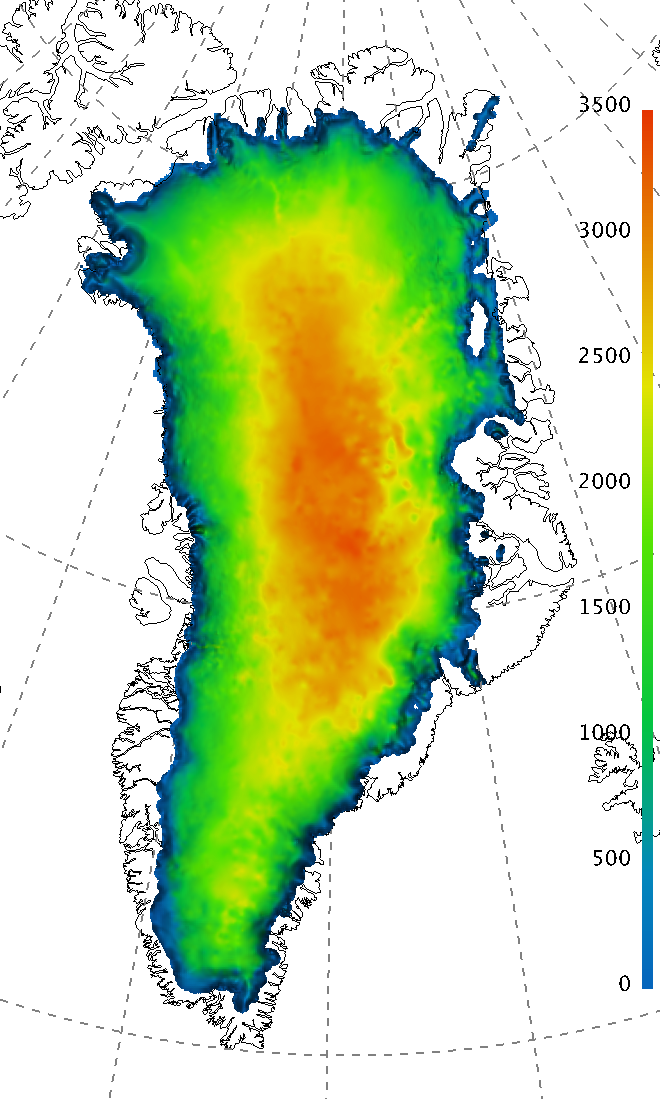
\includegraphics[width=2.0in,keepaspectratio=true]{sr-greenland-thk}
  \qquad
  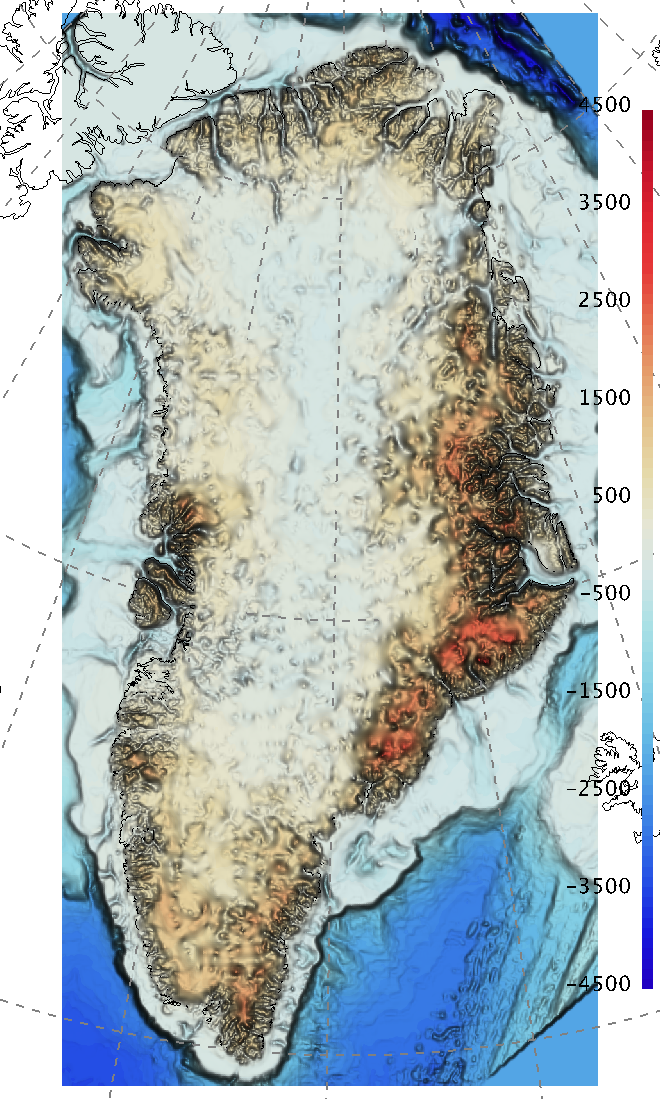
\includegraphics[width=2.0in,keepaspectratio=true]{sr-greenland-topg}
  \qquad
  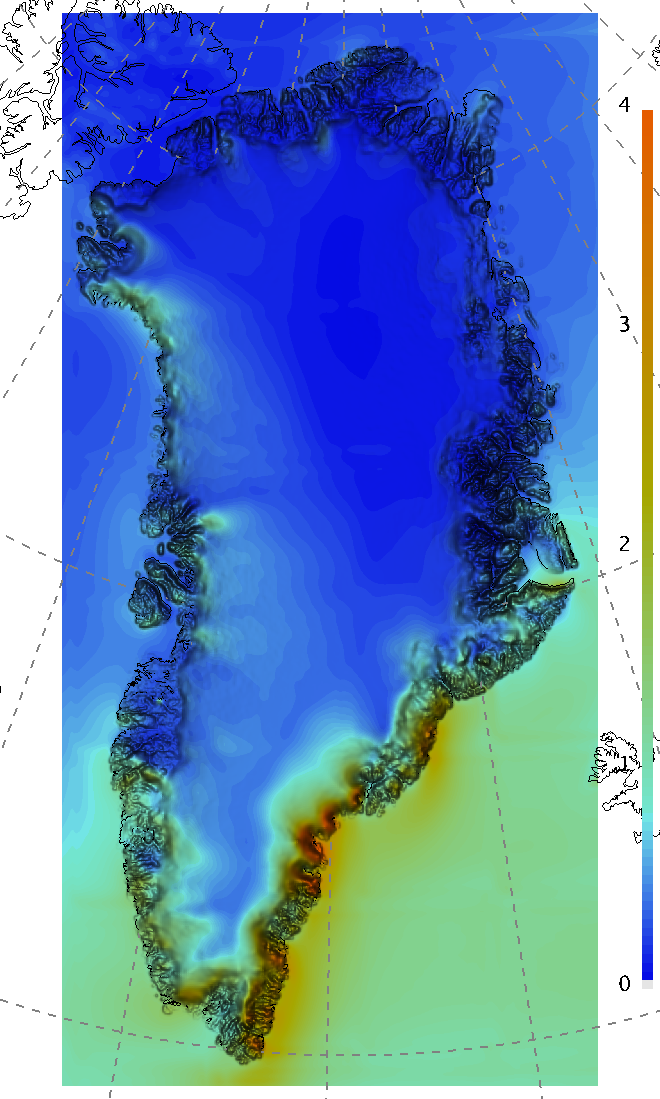
\includegraphics[width=2.0in,keepaspectratio=true]{sr-greenland-prcp}}
\caption{The input file contains present-day ice thickness (left; m), bedrock elevation (center; m), and present-day precipitation (right; m $\text{a}^{-1}$ ice equivalent) for SeaRISE-Greenland.  These are fields \texttt{thk}, \texttt{topg}, and \texttt{precipitation}, respectively, in \texttt{pism_Greenland_5km_v1.1.nc}.}
\label{fig:sr-input}
\end{figure}


\subsection{First run}   \label{subsect:runscript}  Like many Unix programs, PISM allows a lot of command-line options.  In fact, because the variety of allowed ice sheet, shelf, and glacier configurations, and included sub-models, is so large, the list of possible command-line options covers sections \ref{sec:initboot} through \ref{sec:practical-usage} of this manual.  In practice one often builds scripts to run PISM with the correct options, which is what we show here.  The script we use is ``\texttt{spinup.sh}'' in the \texttt{examples/std-greenland/} subdirectory of \texttt{pism/}.

Note that initializing ice sheets, generically called ``spin-up'', can be done by computing approximate steady states with constant boundary data, or, in some cases, by integrating paleo-climatic and long-time-scale information, also applied at the ice sheet boundary, to build a model for the present state of the ice sheet.  Both of these possibilities are illustrated in the \texttt{spinup.sh} script.  The spin-up stage of using an ice sheet model may actually require more processor-hours than follow-on ``experiment'' or ``forecast'' stages.

To see what can be done with the script, read the usage message it produces:
\begin{verbatim}
$ ./spinup.sh
\end{verbatim}

The simplest spin-up approach is to use a ``constant-climate'' model.  We take this approach first.  To see a more detailed view of the PISM command for the first run, do:
\begin{verbatim}
$ PISM_DO=echo ./spinup.sh 4 const 10000 20 sia g20km_10ka.nc
\end{verbatim}
Setting the environment variable \texttt{PISM_DO} in this way tells \texttt{spinup.sh} just to print out the commands it is about to run, not do them.  The ``proposed'' run looks like this:
\label{firstcommand}
\small
\begin{verbatim}
mpiexec -n 4 pismr -i pism_Greenland_5km_v1.1.nc -bootstrap -Mx 76 -My 141 \
  -Mz 101 -Mbz 11 -z_spacing equal -Lz 4000 -Lbz 2000 -skip -skip_max 10 \
  -ys -10000 -ye 0 -surface given -surface_given_file pism_Greenland_5km_v1.1.nc \
  -calving ocean_kill pism_Greenland_5km_v1.1.nc -sia_e 3.0 \
  -ts_file ts_g20km_10ka.nc -ts_times -10000:yearly:0 \
  -extra_file ex_g20km_10ka.nc -extra_times -10000:100:0 \
  -extra_vars diffusivity,temppabase,tempicethk_basal,bmelt,tillwat,velsurf_mag,mask,thk,topg,usurf \
  -o g20km_10ka.nc
\end{verbatim}
\normalsize
Let's briefly deconstruct this run.

At the front is ``\texttt{mpiexec -n 4 pismr}''.  This means that the PISM executable \texttt{pismr} is run in parallel on four processes parallel standard (e.g.~cores) under the Message Passing Interface (``MPI''; \url{http://www.mcs.anl.gov/mpi/}).  Though we are assuming you have a workstation or laptop with at least 4 cores, this example will work with 1 to about 50 processors, with reasonably good scaling in speed.  Scaling can be good with more processors if we run at higher spatial resolution \cite{BBssasliding,DickensMorey2013}.  The executable name ``\texttt{pismr}'' stands for the standard ``run'' mode of PISM (in contrast to specialized modes described later in sections \ref{sec:verif} and \ref{sec:simp}).

Next, the proposed run uses option \texttt{-bootstrap} to start the run by ``bootstrapping.'' This term describes the creation, by heuristics and highly-simplified models, of the mathematical initial conditions required for a deterministic, time-dependent ice dynamics model.  Then the options describe a $76\times 141$ point grid in the horizontal, which gives 20\,km grid spacing in both directions.  Then there are choices about the vertical extent and resolution of the computational grid; more on those later.  After that we see a description of the time-axis, with a start and end time given: ``\texttt{-ys -10000 -ye 0}''.

Then we get the instructions that tell PISM to read the upper surface boundary conditions (i.e.~climate) from a file: ``\texttt{-surface given -surface_given_file pism_Greenland_5km_v1.1.nc}''.  For more on these choices, see subsection \ref{sec:climate-inputs}, and also the PISM Climate Forcing Manual.

Then there are a couple of options related to ice dynamics.  First is a minimal calving model which removes ice at the calving front location given by a thickness field in the input file (``\texttt{-calving ocean_kill}''); see subsection \ref{sec:calving} for this and other calving options).  Then there is a setting for enhanced ice softness (``\texttt{-sia_e 3.0}'').  See subsection \ref{sec:rheology} for more on this enhancement parameter, which we also return to later in the current section in a parameter study.

Then there are longish options describing the fields we want as output, including scalar time series (``\texttt{-ts_file ts_g20km_10ka.nc -ts_times -10000:yearly:0}''; see section \ref{sec:practical-usage}) and space-dependent fields (``\texttt{-extra_file ...}''; again see section \ref{sec:practical-usage}), and finally the named output file (``\texttt{-o g20km_10ka.nc}'').

Note that the modeling choices here are reasonable, but they are not the only way to do it! The user is encouraged to experiment; that is the point of a model.

Now let's actually get the run going:
\begin{verbatim}
$ ./spinup.sh 4 const 10000 20 sia g20km_10ka.nc &> out.g20km_10ka &
\end{verbatim}
\noindent The terminating ``\verb|&|'', which is optional, asks unix to run the command in the background, so we can keep working in the current shell.  Because we have re-directed the text output (``\verb|&> out.g20km_10ka|''), PISM will show what it is doing in the text file \texttt{out.g20km_10ka}.  Using \texttt{less} is a good way to watch such a growing text-output file.  This run should take 20 minutes or less.


\subsection{Watching the first run}  \label{subsect:watchrun}  As soon as the run starts it creates time-dependent NetCDF files \texttt{ts_g20km_10ka.nc} and \texttt{ex_g20km_10ka.nc}.  The latter file, which has spatially-dependent fields at each time, is created after the first 100 model years, a few wall clock seconds in this case.  The command \texttt{-extra_file ex_g20km_10ka.nc -extra_times -10000:100:0} adds a spatially-dependent ``frame'' at model times -9900, -9800, \dots, 0.

To look at the spatial-fields output graphically, do:
\begin{verbatim}
$ ncview ex_g20km_10ka.nc
\end{verbatim}
We see that \texttt{ex_g20km_10ka.nc} contains growing ``movies'' of the fields chosen by the \texttt{-extra_vars} option.  A frame of the ice thickness field \texttt{thk} is shown in Figure \ref{fig:growing} (left).

The time-series file \texttt{ts_g20km_10ka.nc} is also growing.  It contains spatially-averaged ``scalar'' diagnostics like the total ice volume or the ice-sheet-wide maximum velocity (variable \texttt{ivol} and \texttt{max_hor_vel}, respectively).  It can be viewed
\begin{verbatim}
$ ncview ts_g20km_10ka.nc
\end{verbatim}
The growing time series for \texttt{ivol} is shown in Figure \ref{fig:growing} (right).  Recall that our intention was to generate a minimal model of the Greenland ice sheet in approximate steady-state with a steady (constant-in-time) climate.  The measurable steadiness of the \texttt{ivol} time series is a possible standard for steady state \cite[for example]{EISMINT00}.

\begin{figure}[ht]
\centering
\mbox{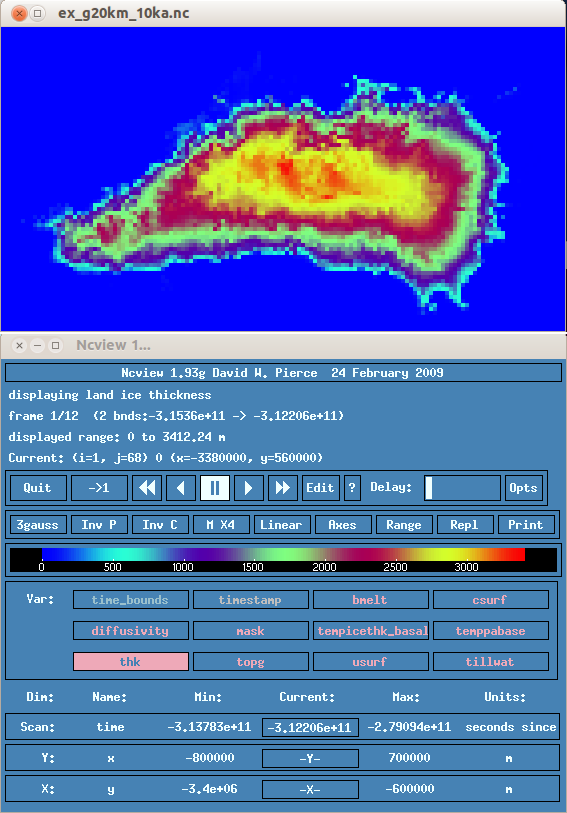
\includegraphics[height=5.0in,keepaspectratio=true]{ex-growing-thk-g20km}
  \qquad 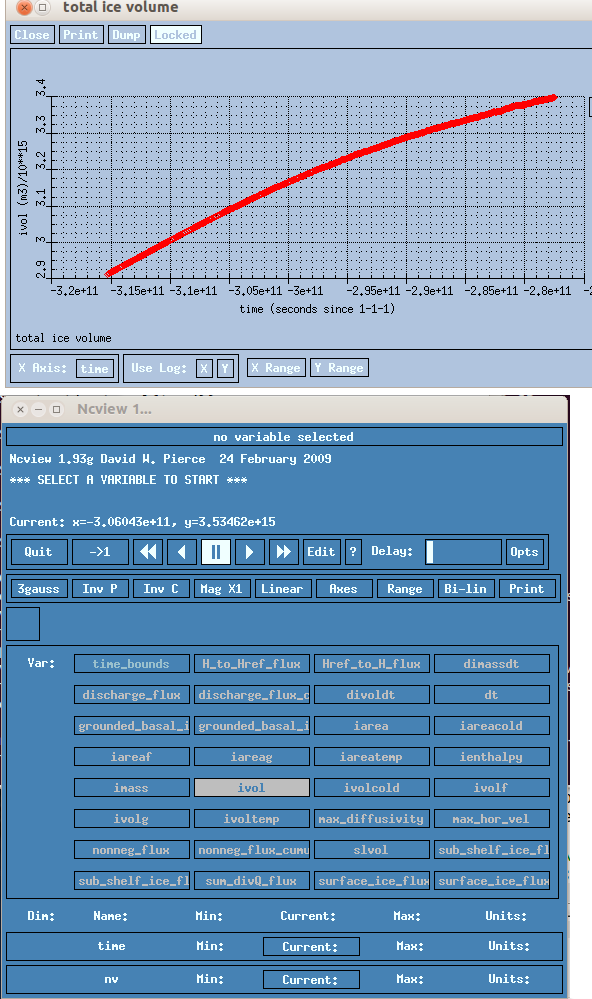
\includegraphics[height=5.0in,keepaspectratio=true]{ts-growing-ivol-g20km}}
\caption{Two views produced by \texttt{ncview} during a PISM model run.  Left: \texttt{thk}, the ice sheet thickness, a space-dependent field, from file \texttt{ex_g20km_10ka.nc}.  Right: \texttt{ivol}, the total ice sheet volume time-series, from file \texttt{ts_g20km_10ka.nc}.}
\label{fig:growing}
\end{figure}

At the end of the run the output file \texttt{g20km_10ka.nc} is generated.  Figure \ref{fig:firstoutput} shows some fields from this file.  In the next subsections we consider their ``quality'' as model results.  To see a report on computational performance, we do:
\begin{verbatim}
$ ncdump -h g20km_10ka.nc |grep history
    :history = "user@machine 2013-11-23 15:57:22 AKST: PISM done.  Performance stats:
0.3435 wall clock hours, 1.3738 proc.-hours, 7274.0065 model years per proc.-hour,
PETSc MFlops = 0.03.\n",
\end{verbatim}

\begin{figure}[ht]
\centering
\mbox{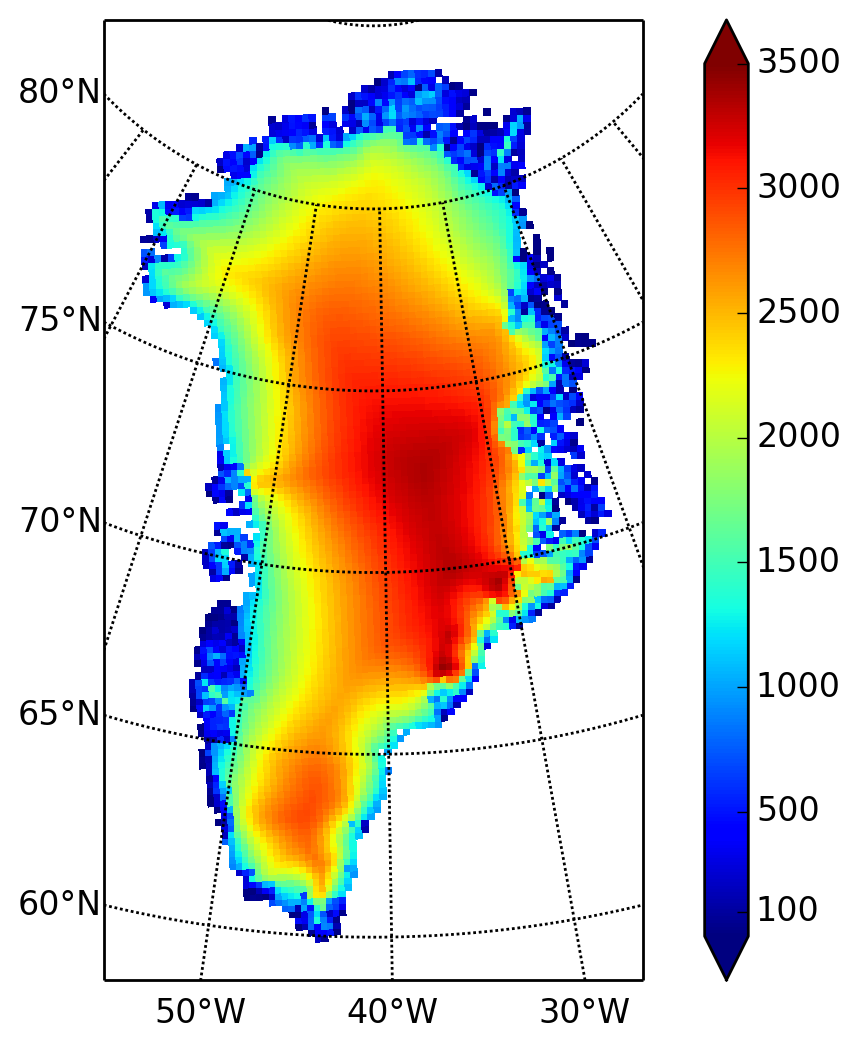
\includegraphics[height=2.75in,keepaspectratio=true]{g20km-10ka-usurf} 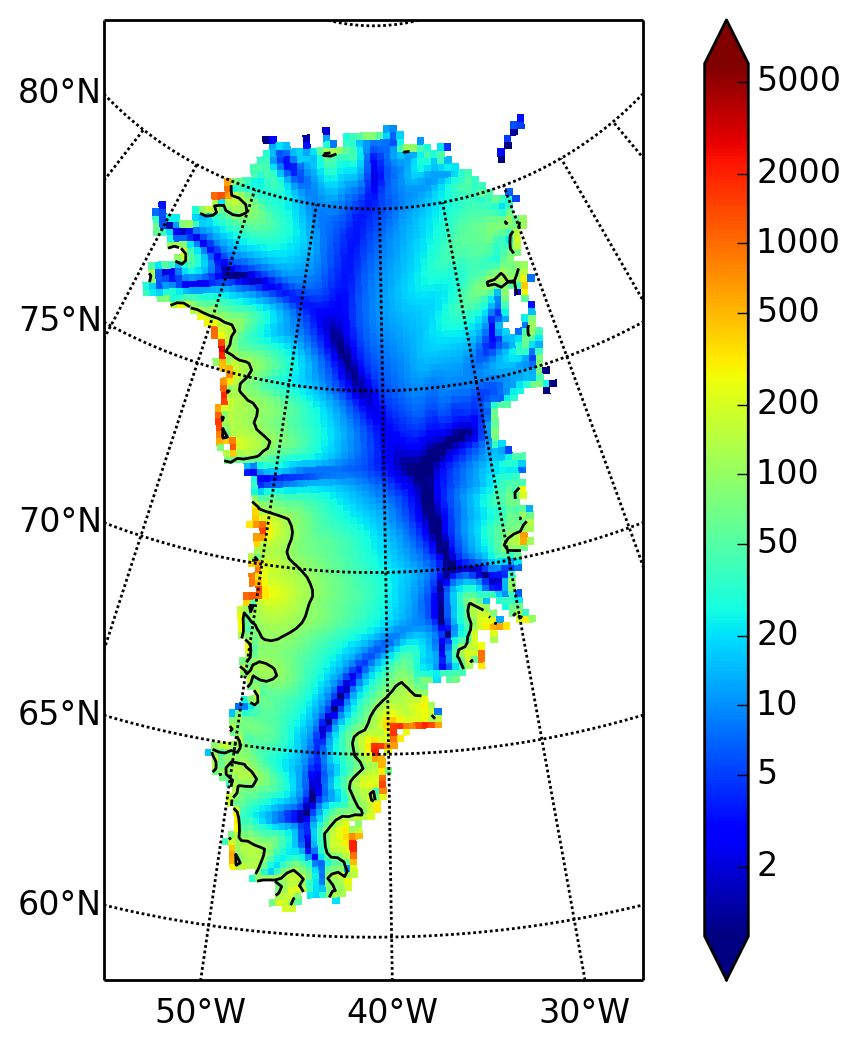
\includegraphics[height=2.75in,keepaspectratio=true]{g20km-10ka-csurf} 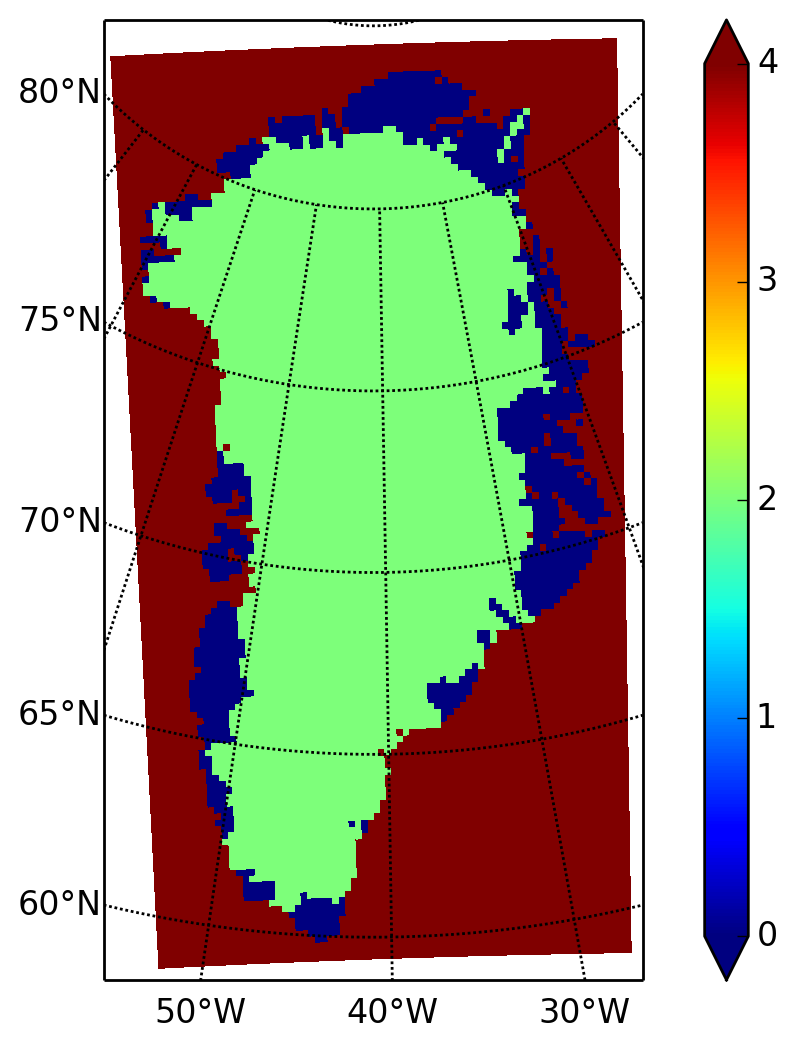
\includegraphics[height=2.75in,keepaspectratio=true]{g20km-10ka-mask}}
\caption{Fields from output file \texttt{g20km_10ka.nc}.  Left: \texttt{usurf}, the ice sheet surface elevation in meters.  Middle: \texttt{velsurf_mag}, the surface speed in meters/year ($=$ m/a), including the 100 m/a contour (solid black).  Right: \texttt{mask}, with 0 = ice-free land, 2 = grounded ice, 4 = ice-free ocean.}
\label{fig:firstoutput}
\end{figure}


\subsection{Second run: a better ice-dynamics model}  \label{subsect:ssarun}

It is widely-understood that ice sheets slide on their bases, especially when liquid water is present at the base (see \cite{Joughinetal2001,MacAyeal}, among others).  An important aspect of modeling such sliding is the inclusion of membrane or ``longitudinal'' stresses into the stress balance \cite{BBssasliding}.  The basic stress balance in PISM which involves membrane stresses is the Shallow Shelf Approximation (SSA) \cite{WeisGreveHutter}.  The stress balance used in the previous section was, by contrast, the (thermomechanically-coupled) non-sliding, non-membrane-stress Shallow Ice Approximation (SIA) \cite{BBL,EISMINT00}.  The preferred ice dynamics model within PISM, that allows both sliding balanced by membrane stresses and shear flow as described by the SIA, is the SIA+SSA ``hybrid'' model \cite{BBssasliding,Winkelmannetal2011}.  For more on stress balance theories see section \ref{sec:dynamics} of this Manual.

The practical issue with models of sliding is that a distinctly-uncertain parameter space must be introduced.  This especially involves parameters controlling the amount and pressure of subglacial water (see \cite{AschwandenAdalgeirsdottirKhroulev,Clarke05,Tulaczyketal2000,vanPeltOerlemans2012} among other references).  In this regard, PISM uses the concept of a saturated and pressurized subglacial till with a modeled distribution of yield stress  \cite{BBssasliding,SchoofStream}.  The yield stress arises from the PISM model of the production of subglacial water, which is itself computed through the conservation of energy model \cite{AschwandenBuelerKhroulevBlatter}.  We use such models in the rest of this Getting Started section.

While the \texttt{spinup.sh} script has default sliding-related parameters, for demonstration purposes we change one parameter.  We replace the default power $q=0.25$ in the sliding law (the equation which relates both the subglacial sliding velocity and the till yield stress to the basal shear stress which appears in the SSA stress balance) by a less ``plastic'' and more ``linear'' choice $q=0.5$.  See subsection \ref{subsect:basestrength} for more on sliding laws.  To see the run we propose, do
\begin{verbatim}
$ PISM_DO=echo PARAM_PPQ=0.5 ./spinup.sh 4 const 10000 20 hybrid g20km_10ka_hy.nc
\end{verbatim}
Now remove ``\texttt{PISM_DO=echo}'' and redirect the text output into a file to start the run:
\begin{verbatim}
$ PARAM_PPQ=0.5 ./spinup.sh 4 const 10000 20 hybrid g20km_10ka_hy.nc &> out.g20km_10ka_hy &
\end{verbatim}
This run should take 30 minutes or less.\footnote{Regarding the relative speeds of the runs that produce \texttt{g20km_10ka.nc} and \texttt{g20km_10ka_hy.nc}, note that the computation of the SSA stress balance is substantially more expensive than the SIA in a per-step sense.  However, the SSA stress balance in combination with the mass continuity equation causes the maximum diffusivity in the ice sheet to be substantially lower during the run.  Because the maximum diffusivity controls the time-step in the PISM adaptive time-stepping scheme \cite{BBL}, the number of time steps is reduced in the hybrid run.  To see this contrast use\, \texttt{ncview ts_g20km_10ka*nc}\, to view variables \texttt{max_diffusivity} and \texttt{dt}.}

When this run is finished it produces \texttt{g20km_10ka_hy.nc}.  As before do
\begin{verbatim}
$ ncdump -h g20km_10ka_hy.nc |grep history
\end{verbatim}
to see performance results for your machine.  The number reported as ``\texttt{PETSc MFlops}'' from this run is about $3 \times 10^5$, much larger than the previous run, because now calls to the PETSc library are used when solving the non-local SSA stress balance in parallel.

The results of this run are shown in Figure \ref{fig:secondoutputcoarse}.  We show the basal sliding speed field \texttt{velbase_mag} in this Figure, where Figure \ref{fig:firstoutput} had the \texttt{mask}, but the reader can check that \texttt{velbase_mag}=0 in the nonsliding SIA-only result \texttt{g20km_10ka.nc}.

\begin{figure}[ht]
\centering
\mbox{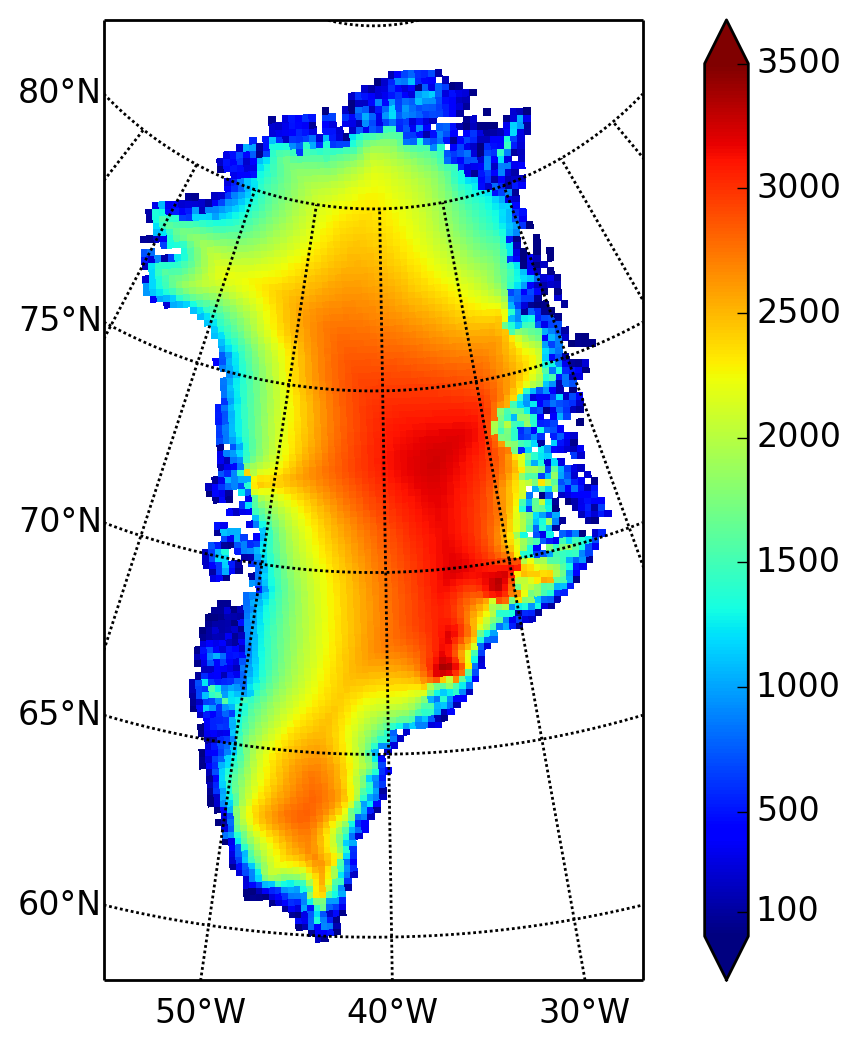
\includegraphics[height=2.75in,keepaspectratio=true]{g20km-10ka-hy-usurf} 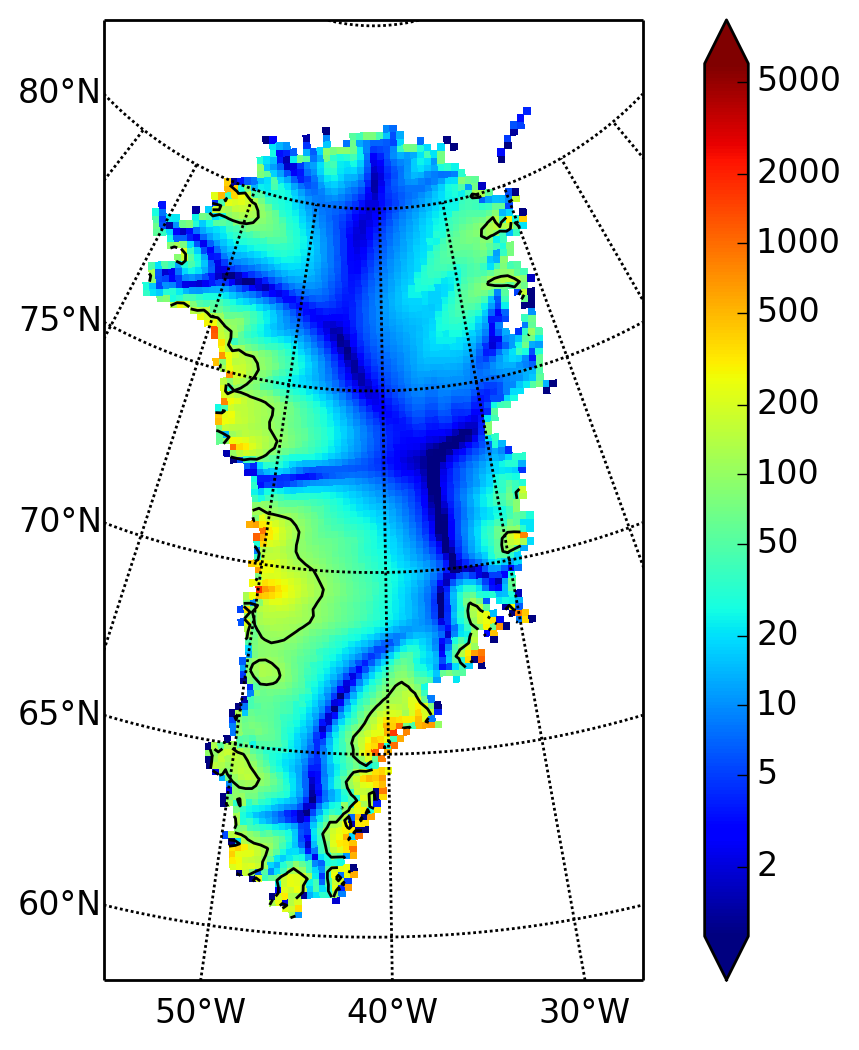
\includegraphics[height=2.75in,keepaspectratio=true]{g20km-10ka-hy-csurf} 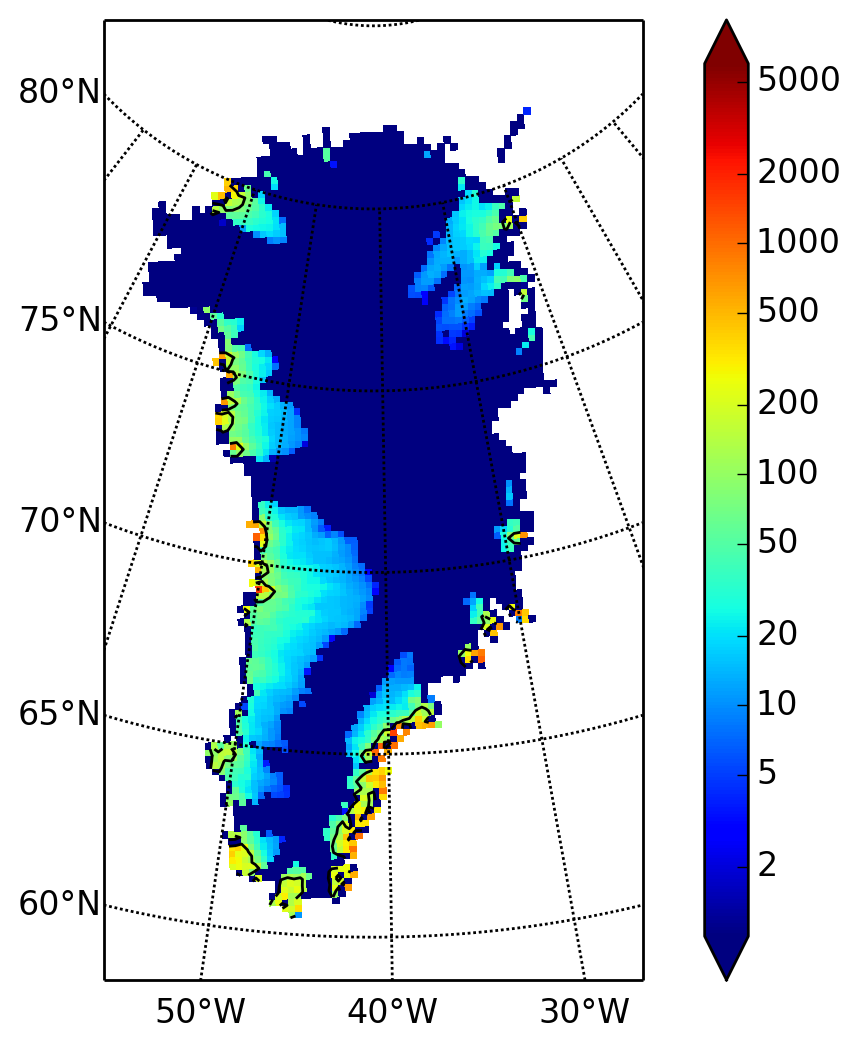
\includegraphics[height=2.75in,keepaspectratio=true]{g20km-10ka-hy-cbase}}
\caption{Fields from output file \texttt{g20km_10ka_hy.nc}.  Left: \texttt{usurf}, the ice sheet surface elevation in meters.  Middle: \texttt{velsurf_mag}, the surface speed in m/a, including the 100 m/a contour (solid black).  Right: the sliding speed \texttt{velbase_mag}, shown the same way as \texttt{velsurf_mag}.}
\label{fig:secondoutputcoarse}
\end{figure}

The hybrid model includes sliding, and it is important to evaluate that aspect of the output.  However, though it is critical to the response of the ice to changes in climate, basal sliding velocity is essentially unobservable in real ice sheets.  On the other hand, because of relatively-recent advances in radar and image technology and processing \cite{Joughin2002}, the surface velocity of an ice sheet is an observable.

So, how good is our model result \texttt{velsurf_mag}?  Figure \ref{fig:csurfvsobserved} compares the radar-observed \texttt{surfvelmag} field in the downloaded SeaRISE-Greenland data file \texttt{Greenland_5km_v1.1.nc} with the just-computed PISM result.  The reader might agree with these broad qualitative judgements:

\begin{figure}[ht]
\centering
\mbox{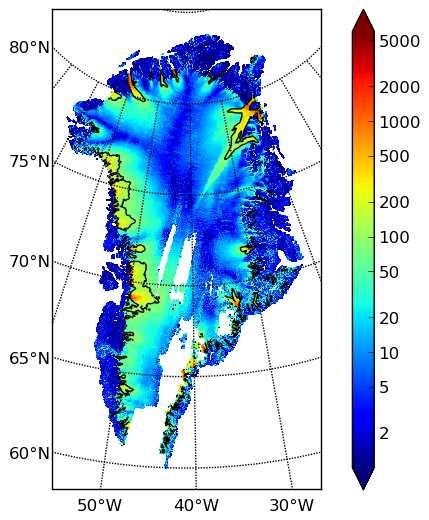
\includegraphics[height=2.75in,keepaspectratio=true]{Greenland-5km-v1p1-surfvelmag} 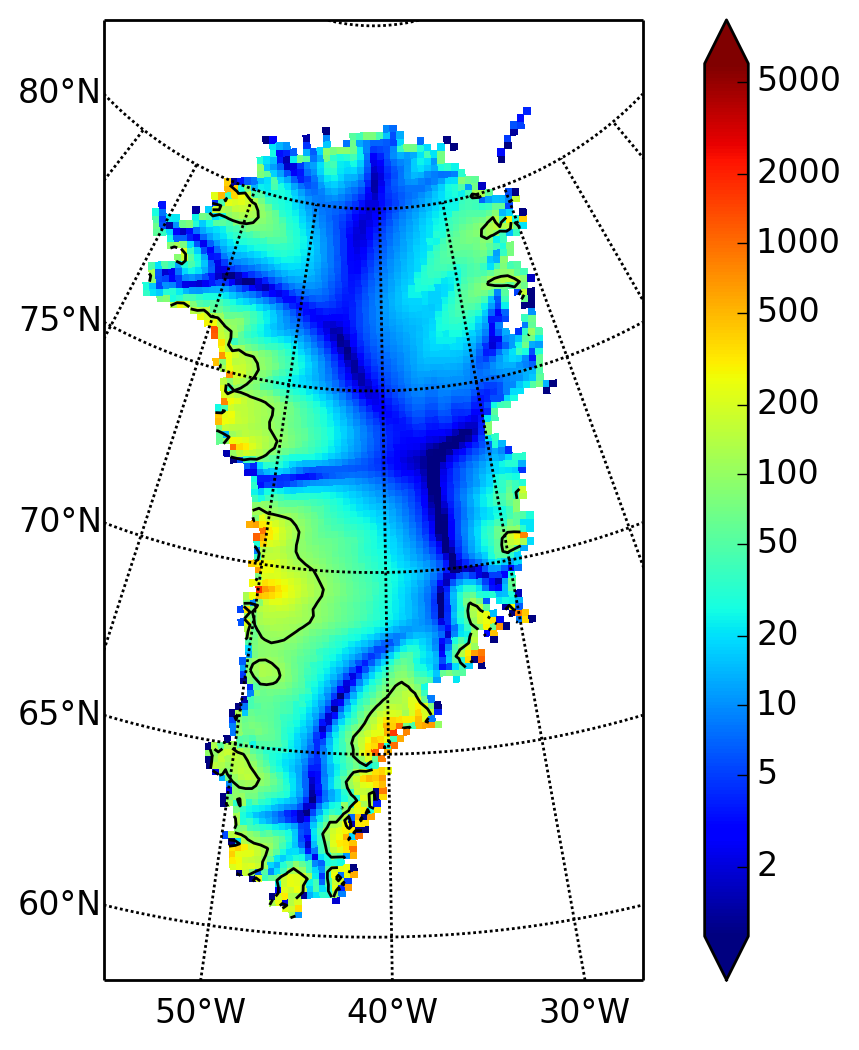
\includegraphics[height=2.75in,keepaspectratio=true]{g20km-10ka-hy-csurf} 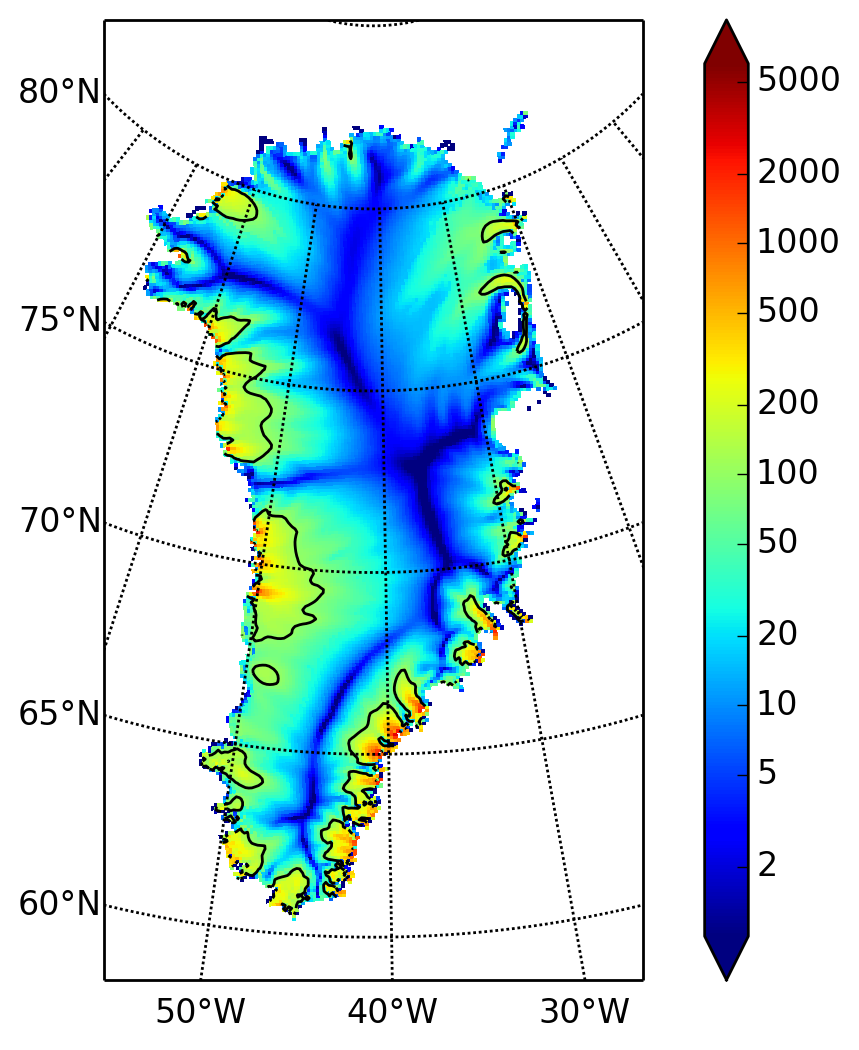
\includegraphics[height=2.75in,keepaspectratio=true]{g10km-10ka-hy-csurf}}
\caption{Comparing observed and modeled surface speed.  All figures have a common scale (m/a), with 100 m/a contour shown (solid black).  Left: \texttt{surfvelmag}, the observed values from SeaRISE data file \texttt{Greenland_5km_v1.1.nc}.  Middle: \texttt{velsurf_mag} from \texttt{g20km_10ka_hy.nc}.  Right: \texttt{velsurf_mag} from \texttt{g10km_10ka_hy.nc}.}
\label{fig:csurfvsobserved}
\end{figure}

\begin{itemize}
\item the model results and the observed surface velocity look similar, and
\item slow near-divide flow is generally in the right areas and of generally the right magnitude, but
\item the observed Northeast Greenland ice stream is more distinct than in the model.
\end{itemize}

We can compare these PISM results to other observed-vs-model comparisons of surface velocity maps, for example Figure 1 in \cite{Priceetal2011} and Figure 8 in \cite{Larouretal2012}.  Only ice-sheet-wide parameters and models were used here in PISM, that is, each location in the ice sheet was modeled by the same physics.  By comparison, those published comparisons involved tuning a large number of subglacial parameters to values which would yield close match to observations of the surface velocity.  Such tuning techniques, called ``inversion'' or ``assimilation'' of the surface velocity data, are also possible in PISM,\footnote{See \cite{vanPeltetal2013} (inversion of DEMs for basal topography) and \cite{Habermannetal2013} (inversion surface velocities for basal shear stress) for PISM-based inversion methods and analysis.} but the advantage of having few parameters in a model is well-known: the results reflect the underlying model not the flexibility of many parameters.

We have only tried two of the many models possible in PISM, and we are free to identify and adjust important parameters.  The first parameter change we consider, in the next subsection, is one of the most important: grid resolution.


\subsection{Third run: higher resolution}  \label{subsect:higherresrun}

Now we change one key parameter, the grid resolution.  Model results differ even when the only change is the resolution.  Using higher resolution ``picks up'' more detail in the bed elevation and climate data.

If you can let it run overnight, do
\begin{verbatim}
$ PARAM_PPQ=0.5 ./spinup.sh 4 const 10000 10 hybrid g10km_10ka_hy.nc &> out.g10km_10ka_hy &
\end{verbatim}
This run might take 4 to 6 hours.  However, supposing you have a larger parallel computer, you can change ``\texttt{mpiexec -n 4}'' to ``\texttt{mpiexec -n N}'' where \texttt{N} is a substantially larger number, up to 100 or so with an expectation of reasonable scaling on this grid \cite{BBssasliding,DickensMorey2013}.

\begin{figure}[ht]
\centering
\mbox{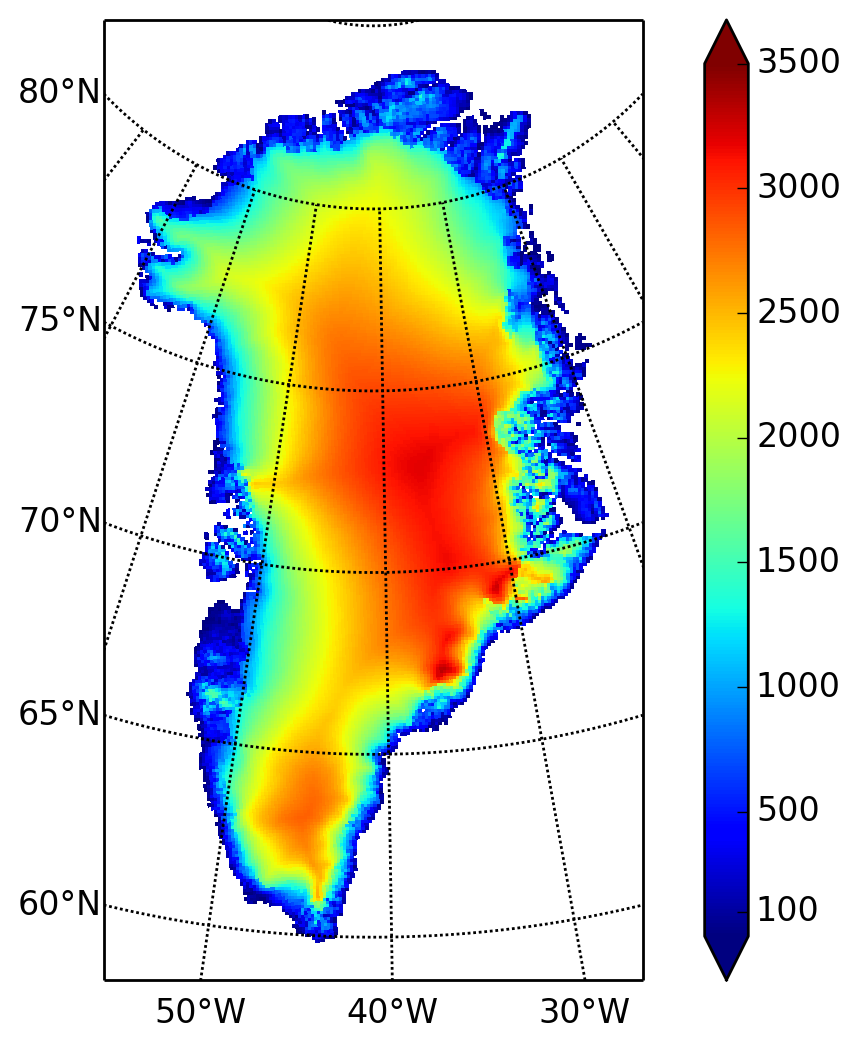
\includegraphics[height=2.75in,keepaspectratio=true]{g10km-10ka-hy-usurf} 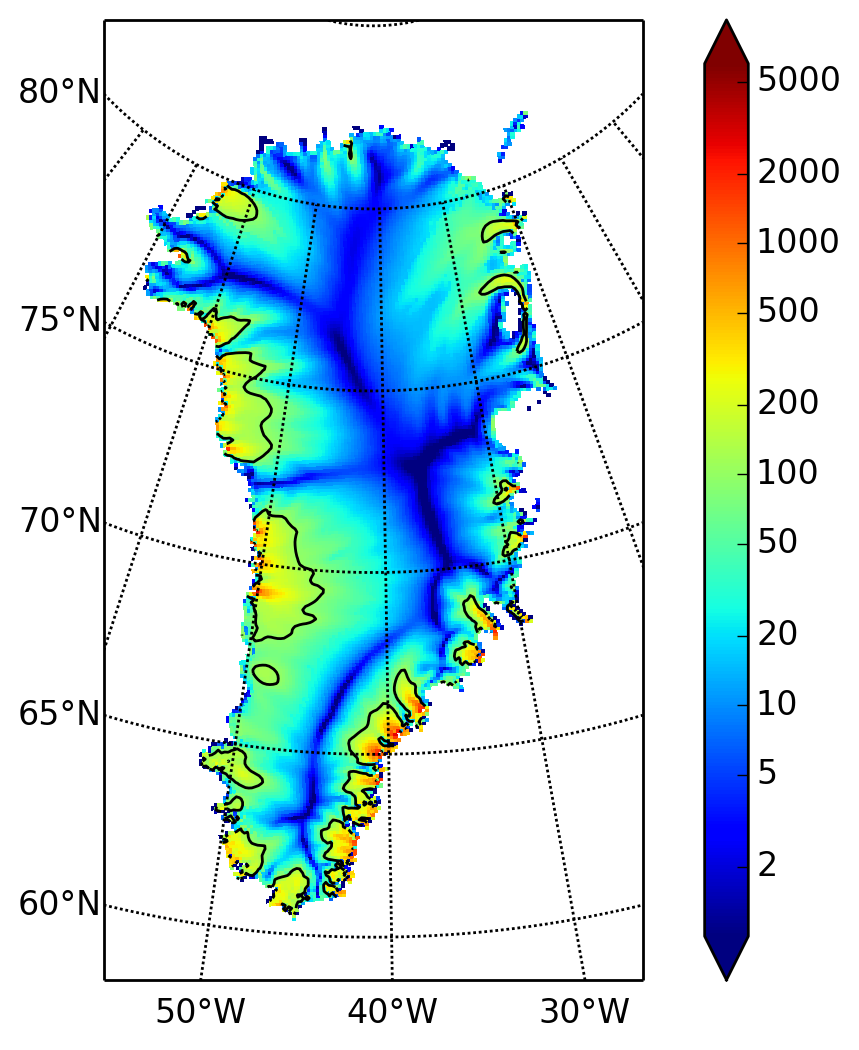
\includegraphics[height=2.75in,keepaspectratio=true]{g10km-10ka-hy-csurf} 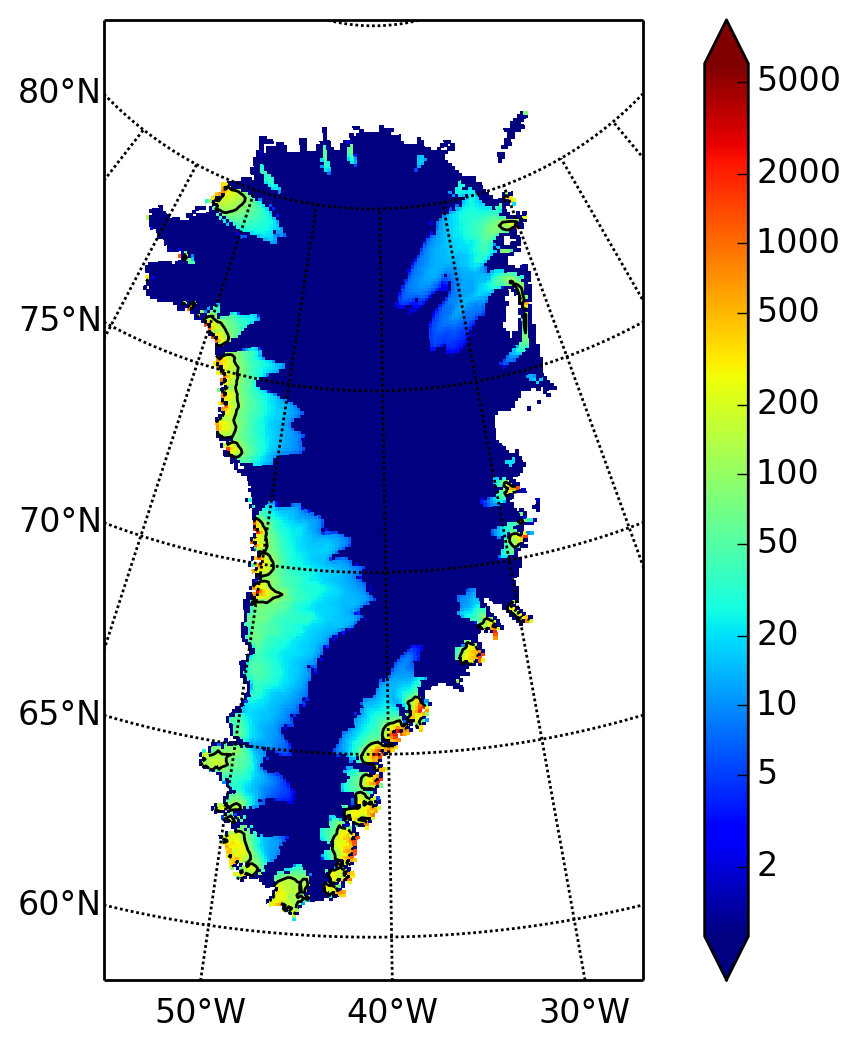
\includegraphics[height=2.75in,keepaspectratio=true]{g10km-10ka-hy-cbase}}
\caption{Fields from output file \texttt{g10km_10ka_hy.nc}.  Compare Figure \ref{fig:secondoutputcoarse}, which only differs by resolution.  Left: \texttt{usurf} in meters.  Middle: \texttt{velsurf_mag} in m/a.  Right: \texttt{velbase_mag} in m/a.}
\label{fig:secondoutputfiner}
\end{figure}

Some fields from the result \verb|g10km_10ka_hy.nc| are shown in Figure \ref{fig:secondoutputfiner}.  Figure \ref{fig:csurfvsobserved} also compares observed velocity to the model results from 20\,km and 10\,km grids.  As a different comparison, Figure \ref{fig:ivolboth} shows ice volume time series \texttt{ivol} for 20\,km and 10\,km runs done here.  We see that this result depends on resolution, in particular because higher resolution grids allow the model to better resolve the flux through topographically-controlled outlet glaciers (compare \cite{Pfefferetal2008}).  However, because the total ice sheet volume is a highly-averaged quantity, the \texttt{ivol} difference from 20\,km and 10\,km resolution runs is only about one part in 60 (about 1.5\%) at the final time.  By contrast, as is seen in the near-margin ice in various locations shown in Figure \ref{fig:csurfvsobserved}, the ice velocity at a particular location may change by 100\% when the resolution changes from 20\,km to 10\,km.

Roughly speaking, the reader should only consider trusting those model results which are demonstrated to be robust across a range of model parameters, and, in particular, which are shown to be relatively-stable among relatively-high resolution results for a particular case.  Using a supercomputer is justified merely to confirm that lower-resolution runs were already ``getting'' a given feature or result.

\begin{figure}[ht]
\centering
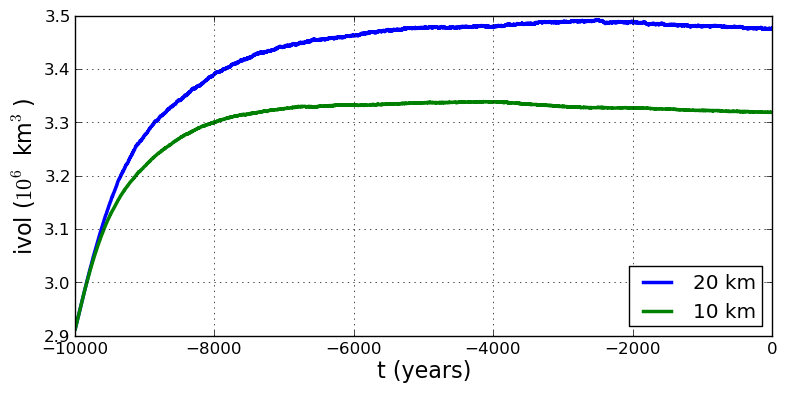
\includegraphics[width=4.0in,keepaspectratio=true]{ivol-both-g20km-g10km}
\caption{Time series of modeled ice sheet volume \texttt{ivol} on 20km and 10km grids.  The present-day ice sheet has volume about $2.9\times 10^6\,\text{km}^3$ \cite{BamberLayberryGogenini}, the initial value seen in both runs.}
\label{fig:ivolboth}
\end{figure}


\subsection{Fourth run: paleo-climate model spin-up}  \label{subsect:paleorun}  

A this point we have barely mentioned one of the most important players in an ice sheet model: the surface mass balance (SMB) model.  Specifically, an SMB model combines precipitation (e.g.~\cite{Balesetal2001} for present-day Greenland) and a model for melt.  Melt models are always based on some approximation of the energy available at the ice surface \cite{Hock05}.  Previous runs in this section used a ``constant-climate'' assumption, which specifically meant using the modeled present-day SMB rates from the regional climate model RACMO \cite{Ettemaetal2009}, as contained in the SeaRISE-Greenland data set \verb|Greenland_5km_v1.1.nc|.

While a physical model of ice dynamics only describes the movement of the ice, the SMB (and the sub-shelf melt rate) are key inputs which directly determine changes in the boundary geometry.  Boundary geometry changes then feedback to determine the stresses seen by the stress balance and thus the motion.

There are other methods for producing SMB than using present-day modeled values.  We now try such a method, a ``paleo-climate spin-up'' for our Greenland ice sheet model.  Of course, direct measurements of prior climates in Greenland are not available as data!  There are, however, estimates of past surface temperatures at the locations of ice cores \cite[for GRIP]{JohnsenetalGRIP}, along with estimates of past global sea level \cite{Imbrieetal1984} which can be used to determine where the flotation criterion is applied---this is how PISM's \verb|mask| variable is determined.  Also, models have been constructed for how precipitation differs from the present-day values \cite{Huybrechts02}.  For demonstration purposes, these are all used in the next run.  The relevant options are further documented in PISM's Climate Forcing Manual.

As noted, one must compute melt in order to compute SMB.  Here this is done using a temperature-index, ``positive degree-day'' (PDD) model \cite{Hock05}.  Such a PDD model has parameters for how much snow and/or ice is melted when surface temperatures spend time near or above zero degrees.  Again, see the PISM Climate Forcing Manual for relevant options.

To summarize the paleo-climate model applied here, temperature offsets from the GRIP core record affect the snow energy balance, and thus the rates of melting and runoff calculated by the PDD model.  In warm periods there is more marginal ablation, but precipitation may also increase (according to a temperature-offset model \cite{Huybrechts02}).  Additionally sea level undergoes changes in time and this affects which ice is floating.  Finally we add an earth deformation model, which responds to changes in ice load by changing the bedrock elevation \cite{BLKfastearth}.

To see how all this translates into PISM options, do
\begin{verbatim}
$ PISM_DO=echo PARAM_PPQ=0.5 REGRIDFILE=g20km_10ka_hy.nc \
  ./spinup.sh 4 paleo 25000 20 hybrid g20km_25ka_paleo.nc
\end{verbatim}

\begin{figure}[ht]
\centering
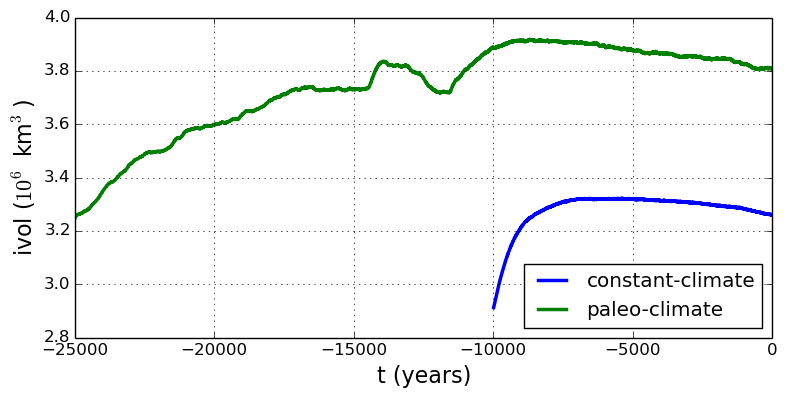
\includegraphics[width=4.5in,keepaspectratio=true]{ivol-const-paleo}
\caption{Time series of modeled ice sheet volume \texttt{ivol} from constant-climate (blue; \texttt{ts_g20km_10ka_hy.nc}) and paleo-climate (red; \texttt{ts_g20km_25ka_paleo.nc}) spinup runs.  Note that the paleo-climate run started with the ice geometry at the end of the constant-climate run.}
\label{fig:ivolconstpaleo}
\end{figure}

You will see an impressively-long command, which you can compare to the one on page \pageref{firstcommand}.  There are several key changes.  First, we do not start from scratch but instead from a previously computed near-equilibrium result:
\begin{verbatim}
  -regrid_file g20km_10ka_hy.nc -regrid_vars litho_temp,thk,enthalpy,tillwat,bmelt
\end{verbatim}
For more on regridding see subsection \ref{sec:regridding}.  Then we turn on the earth deformation model with option \verb|-bed_def lc|; see subsection \ref{subsect:beddef}.  After that the atmosphere and surface (PDD) models are turned on and the files they need are identified:
\begin{verbatim}
  -atmosphere searise_greenland,delta_T,paleo_precip -surface pdd \
  -atmosphere_paleo_precip_file pism_dT.nc -atmosphere_delta_T_file pism_dT.nc
\end{verbatim}
Then the ocean model, which provides both a subshelf melt rate and a time-dependent sealevel to the ice dynamics core, is turned on with \verb|-ocean constant,delta_SL| and the file it needs is identified with \verb|-ocean_delta_SL_file pism_dSL.nc|.  For all of these ``forcing'' options, see the PISM Climate Forcing Manual.  The remainder of the options are similar or identical to the run that created \verb|g20km_10ka_hy.nc|.

To actually start the run, which we rather arbitrarily start at year -25000, essentially at the LGM, do:
\begin{verbatim}
$ PARAM_PPQ=0.5 REGRIDFILE=g20km_10ka_hy.nc \
  ./spinup.sh 4 paleo 25000 20 hybrid g20km_25ka_paleo.nc &> out.g20km_25ka_paleo &
\end{verbatim}
This run should only take one or two hours, noting it is at a coarse 20\,km resolution.

The fields \texttt{usurf}, \texttt{velsurf_mag}, and \texttt{velbase_mag} from file \texttt{g20km_25ka_paleo.nc} are sufficiently similar to those shown in Figure \ref{fig:secondoutputcoarse} that they are not shown here.  Close inspection reveals differences, but of course these runs only differ in the applied climate and run duration and not in resolution or ice dynamics parameters.

\begin{figure}[ht]
\centering
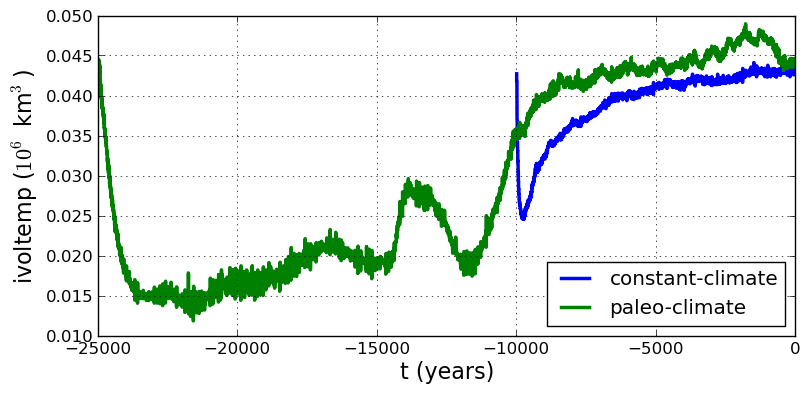
\includegraphics[width=4.5in,keepaspectratio=true]{ivoltemp-const-paleo}
\caption{Time series of temperate ice volume \texttt{ivoltemp} from constant-climate (blue; \texttt{ts_g20km_10ka_hy.nc}) and paleo-climate (red; \texttt{ts_g20km_25ka_paleo.nc}) spinup runs.  The cold of the last ice age affects the fraction of temperate ice.  Note different volume scale compared to that in Figure \ref{fig:ivolconstpaleo}; only about 1\% of ice is temperate (by volume).}
\label{fig:ivoltempconstpaleo}
\end{figure}

To see the difference between runs more clearly, Figure \ref{fig:ivolconstpaleo} compares the time-series variable \texttt{ivol}.  We see the effect of option \verb|-regrid_file g20km_10ka_hy.nc -regrid_vars ...,thk,...|, which implies that the paleo-climate run starts with the ice geometry from the end of the constant-climate run.

Another time-series comparison, of the variable \verb|ivoltemp|, the total volume of temperate (at 0$^\circ$C) ice, appears in Figure \ref{fig:ivoltempconstpaleo}.  The paleo-climate run shows the cold period from $\approx -25$ ka to $\approx -12$ ka.  Both constant-climate and paleo-climate runs then come into rough equilibrium in the holocene.  The bootstrapping artifact, seen at the start of the constant-climate run, which disappears in less than 1000 years, is avoided in the paleo-climate run by starting with the constant-climate end-state.  The reader is encouraged to examine the diagnostic files \texttt{ts_g20km_25ka_paleo.nc} and \texttt{ex_g20km_25ka_paleo.nc} to find more evidence of the (modeled) climate impact on the ice dynamics.


\subsection{Getting serious I: grid sequencing}  \label{subsect:gridseq}  

The previous sections were not very ambitious.  We were just getting started!  Now we demonstrate a serious PISM capability, the ability to change, specifically to \emph{refine}, the grid resolution at runtime.

One can of course do the longest model runs using a coarse grid, like the 20\,km grid used first.  It is, however, only possible to pick up detail from high quality data, for instance bed elevation and/or high-resolution climate data, using high grid resolution.

A 20 or 10\,km grid is inadequate for resolving the flow of the ice sheet through the kind of fjord-like, few-kilometer-wide topographical confinement which occurs, for example, at Jakobshavn Isbrae in the west Greenland ice sheet \cite{Joughinetal08}, an important outlet glacier which both flows fast and drains a large fraction of the ice sheet.  One possibility is to set up an even higher-resolution PISM regional model covering only one outlet glacier, but this requires decisions about coupling to the whole ice sheet flow.  (See section \ref{sec:jako}.)  But here we will work on high resolution for the whole ice sheet, and thus all outlet glaciers.

Consider the following command; compare it to the one on page \pageref{firstcommand}:
\begin{verbatim}
mpiexec -n 4 pismr -i pism_Greenland_5km_v1.1.nc -bootstrap -Mx 301 -My 561 \
  -Mz 201 -Mbz 21 -z_spacing equal -Lz 4000 -Lbz 2000 -ys -200 -ye 0 \
  -regrid_file g20km_10ka_hy.nc -regrid_vars litho_temp,thk,enthalpy,tillwat,bmelt ...
\end{verbatim}
Instead of a 20\,km grid in the horizontal (\verb|-Mx 76 -My 141|) we ask for a 5\,km grid (\verb|-Mx 301 -My 561|).  Instead of vertical grid resolution of 40\,m (\verb|-Mz 101 -z_spacing equal -Lz 4000|) we ask for a vertical resolution of 20\,m (\verb|-Mz 201 -z_spacing equal -Lz 4000|).\footnote{See subsections \ref{sec:bootstrapping}, \ref{subsect:coords}, and \ref{subsect:grid} for more about determining the computation domain and grid at bootstrapping.}  Most significantly, however, we say \verb|-regrid_file g20km_10ka_hy.nc| to regrid---specifically, to bilinearly-interpolate---fields from a model result computed on the coarser 20\,km grid.  The regridded fields (\verb|-regrid_vars litho_temp,...|) are the evolving mass and energy state variables which are already approximately at equilibrium on the coarse grid.  Because we are bootstrapping (i.e.~using the \texttt{-bootstrap} option), the other variables, especially the bedrock topography \verb|topg| and the climate data, are brought in to PISM at ``full'' resolution, that is, on the original 5\,km grid in the data file \texttt{pism_Greenland_5km_v1.1.nc}.

This technique could be called ``grid sequencing''.\footnote{It is not quite ``multigrid.''  That would both involve refinement and coarsening stages in computing the fine grid solution.}  The result of the above command will be to compute the near-equilibrium result on the fine 5\,km grid, taking advantage of the coarse-gridded computation of approximate equilibrium, and despite a run of only 200 model years (\verb|-ys -200 -ye 0|).  How close to equilibrium we get depends on both durations, i.e.~on both the coarse and fine grid run durations, but certainly the computational effort is reduced by doing a short run on the fine grid.  Note that in the previous subsection we also used regridding.  In that application, however, \verb|-regrid_file| only ``brings in'' fields from a run on the same resolution.

Generally the fine grid run duration in grid sequencing should be at least $t = \Delta x / v_{\text{min}}$ where $\Delta x$ is the fine grid resolution and $v_{\text{min}}$ is the lowest ice flow speed that we expect to be relevant to our modeling purposes.  That is, the duration should be such that slow ice at least has a chance to cross one grid cell.  In this case, if $\Delta x = 5$\,km and $v_{\text{min}} = 25$\,m/a then we get $t=200$\,a.  Though we use this as the duration, it is a bit short, and the reader might compare $t=500$ results (i.e.~using $v_{\text{min}} = 10$\,m/a).

Actually we will demonstrate how to go from $20\,\text{km}$ to $5\,\text{km}$ in two steps, $20\,\text{km}\,\to\,10\,\text{km}\,\to\,5\,\text{km}$, with durations of 10\,ka, 2\,ka, and 200\,a, respectively.  The 20\,km coarse grid run is already done; the result is in \texttt{g20km_10ka_hy.nc}.  So we run the following script which is \texttt{gridseq.sh} in \texttt{examples/std-greenland/}.  It calls \texttt{spinup.sh} to collect all the right PISM options:
\begin{scriptvrb}
#!/bin/bash
NN=4
export PARAM_PPQ=0.5
export REGRIDFILE=g20km_10ka_hy.nc
export EXSTEP=100
./spinup.sh $NN const 2000  10 hybrid g10km_gridseq.nc
export REGRIDFILE=g10km_gridseq.nc
export EXSTEP=10
./spinup.sh $NN const 200    5 hybrid  g5km_gridseq.nc
\end{scriptvrb}
Environment variable \verb|EXSTEP| specifies the time in years between writing the spatially-dependent, and large-file-size-generating, frames for the \verb|-extra_file ...| diagnostic output.

Before you run the above script, however, an important

\medskip
\centerline{\large\underline{\emph{WARNING:} the 5\,km run requires 8\,Gb of memory at minimum!}\normalsize}

\medskip
\noindent If you try it without at least 8 Gb of memory then your machine will ``bog down'' and start using the hard disk for swap space!  The run will not complete and your hard disk will get a lot of wear!  (If you have less than 8 Gb memory, comment out the last three lines of the above script---e.g.~using the ``\verb|#|'' character at the beginning of the line---so that you only do the 20\,km $\to$ 10\,km refinement.)

Run the script like this:
\begin{verbatim}
$ ./gridseq.sh &> out.gridseq &
\end{verbatim}
The 10\,km run takes under two wall-clock hours (8 processor-hours) and the 5\,km run takes about 6 wall-clock hours (24 processor-hours).

\begin{figure}[ht]
\centering
\mbox{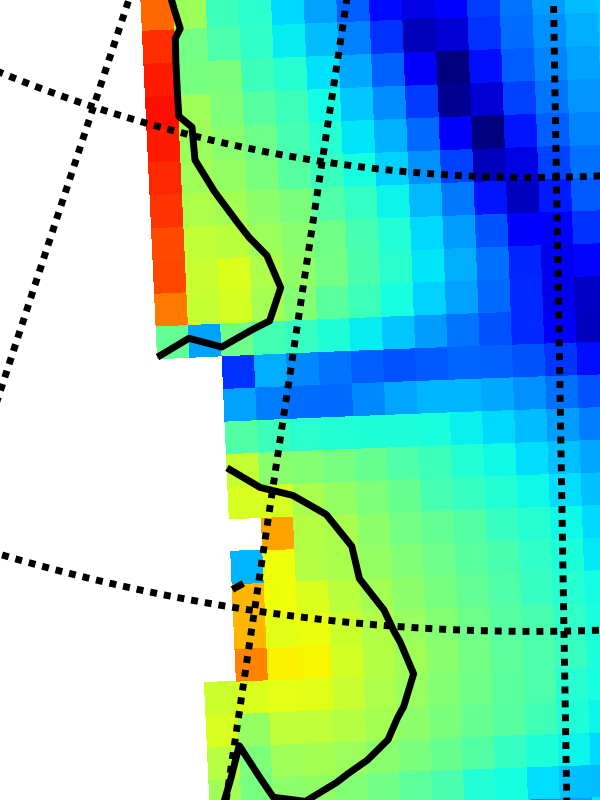
\includegraphics[width=1.65in,keepaspectratio=true]{g40km-detail} 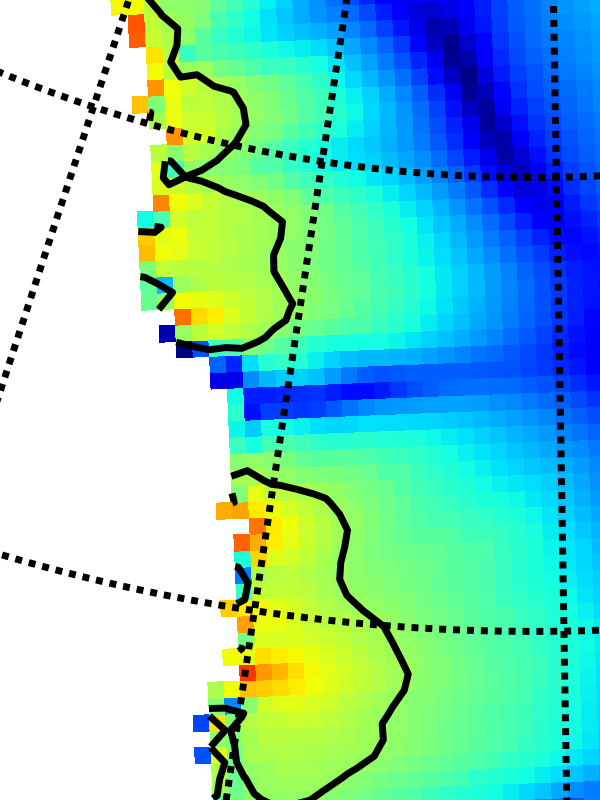
\includegraphics[width=1.65in,keepaspectratio=true]{g20km-detail} 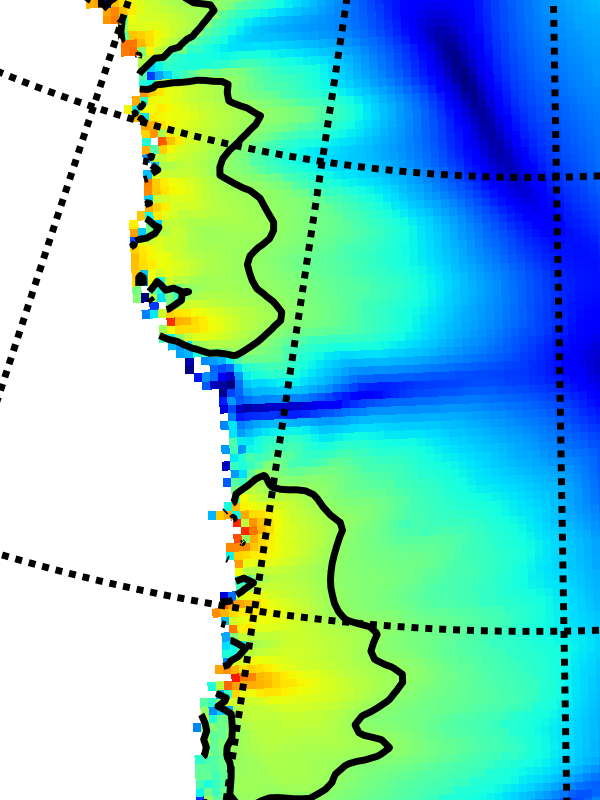
\includegraphics[width=1.65in,keepaspectratio=true]{g10km-detail} 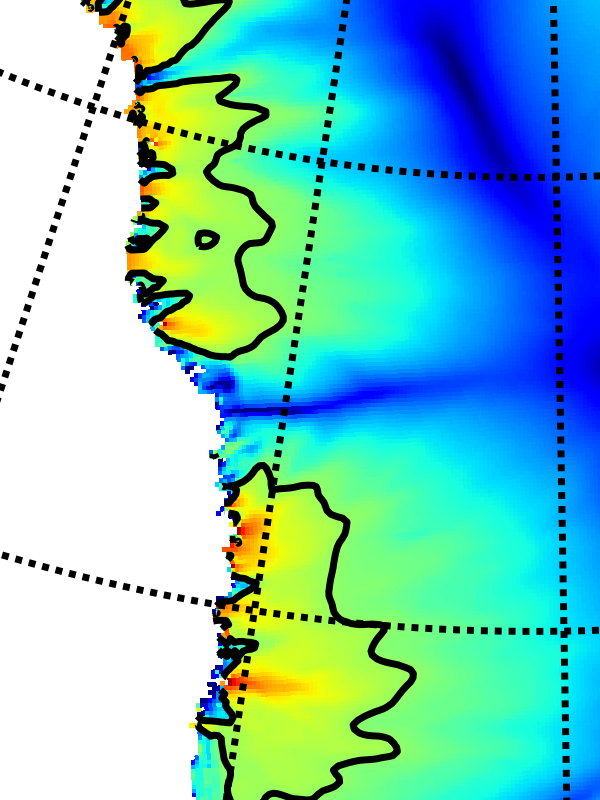
\includegraphics[width=1.65in,keepaspectratio=true]{g5km-detail} }
\caption{Detail of field \texttt{velsurf_mag} showing the central western coast of Greenland, including Jakobshavn Isbrae (lowest major flow), from runs of resolution 40, 20, 10, 5\,km (left-to-right).  Color scheme and scale, including 100\,m/a contour (solid black), are all identical to \texttt{velsurf_mag} Figures \ref{fig:secondoutputcoarse}, \ref{fig:csurfvsobserved}, and \ref{fig:secondoutputfiner}.}
\label{fig:gridseqdetail}
\end{figure}

Figure \ref{fig:gridseqdetail}, showing only a detail of the western coast of Greenland, with several outlet glaciers visible, suggests what is accomplished: the high resolution runs have separated outlet glacier flows, as they are in fact.  Note that all of these results were generated in a few wall clock hours on a laptop!  The surface speed \texttt{velsurf_mag} from files \texttt{g10km_gridseq.nc} and \texttt{g5km_gridseq.nc} is shown (two right-most subfigures).  In the two left-hand subfigures we show the same field from NetCDF files \texttt{g40km_10ka_hy.nc} and \texttt{g20km_10ka_hy.nc}; the former is an added 40\,km result using an obvious modification of the run in section \ref{subsect:ssarun}.

\begin{figure}[ht]
\centering
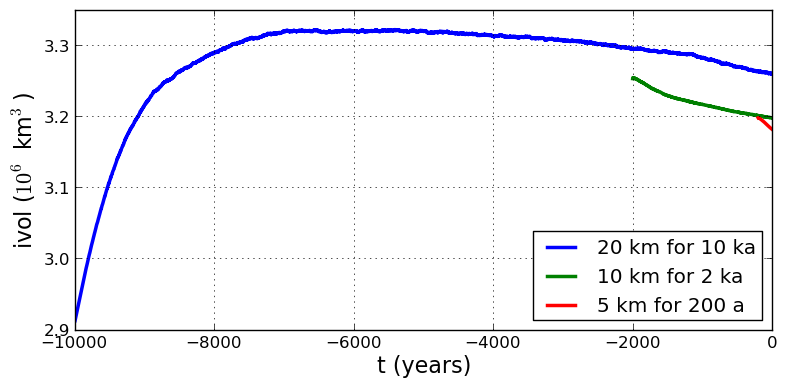
\includegraphics[width=4.5in,keepaspectratio=true]{ivol-gridseq}
\caption{Time series of ice volume \texttt{ivol} from the three runs in our grid sequencing example: 20\,km for 10\,ka = \texttt{ts_g20km_10ka_hy.nc}, 10\,km for 2\,ka = \texttt{ts_g10km_gridseq.nc}, and 5\,km for 200\,a = \texttt{ts_g5km_gridseq.nc}.}
\label{fig:ivolgridseq}
\end{figure}

Figure \ref{fig:ivolgridseq}, which shows time series of ice volume, also shows the cost of high resolution, however.  The short 200\,a run on the 5\,km grid took about 3 wall-clock hours compared to the 10 minutes taken by the 10\,ka run on a 20\,km grid.  The fact that the time series for ice volume on 10\,km and 5\,km grids are not very ``steady'' also suggests that these runs should actually be longer.

In this vein, if you have an available supercomputer then a good exercise is to extend our grid sequencing example to 3\,km or 2\,km resolutions \cite{AschwandenAdalgeirsdottirKhroulev}; these grids are already supported in the script \texttt{spinup.sh}.  Note that the vertical grid also generally gets refined as the horizontal grid is refined.

Going to a 1km grid is possible, but you will start to see the limitations of distributed file systems in writing the enormous NetCDF files in question \cite{DickensMorey2013}.  Notice that a factor-of-five refinement in all three dimensions, e.g.~from 5\,km to 1\,km in the horizontal, and from 20\,m to 4\,m in the vertical, generates an output NetCDF file which is 125 times larger.  Since the already-generated 5 km result \texttt{g5km_gridseq.nc} is over 0.5\,Gb, the result is a very large file at 1\,km.

On the other hand, on fine grids we observe that \emph{memory} parallelism, i.e.~spreading the stored model state over the separated memory of many nodes of supercomputers, is as important as the usual \emph{computation} (CPU) parallelism.

This subsection has emphasized the ``P'' in PISM, the nontrivial parallelism in which the solution of the conservation equations, especially the stress balance equations, is distributed across processors.  An easier and more common mode of parallelism is to distribute distinct model runs, each with different parameter values, among the processors.  For scientific purposes, such parameter studies, whether parallel or not, are at least as valuable as individual high-resolution runs.


\subsection{Getting serious II: an ice dynamics parameter study}  \label{subsect:paramstudy}

The readers of this manual should not assume the PISM authors know all the correct parameters for describing ice flow.  While PISM must have \emph{default} values of all parameters, to help users get started,\footnote{They are stored in human-readable form in the file \texttt{src/pism_config.cdl}.} it has more than two hundred user-configurable parameters.  The goal in this manual is to help the reader adjust them to their desired values.  While ``correct'' values may never be known, or may not exist, examining the behavior of the model as it depends on parameters is both a nontrivial and an essential task.

For some parameters used by PISM, changing their values within their ranges of experimental uncertainty is unlikely to affect model results in any important manner (e.g.~\texttt{sea_water_density}).  For others, however, for instance for the exponent in the basal sliding law, changing the value is highly-significant to model results, as we'll see in this subsection.  This is also a parameter which is very uncertain given current glaciological understanding \cite{CuffeyPaterson}.

To illustrate a parameter study in this Manual we restrict consideration to just two important parameters for ice dynamics,\begin{itemize}
\item $q=$ \texttt{pseudo_plastic_q}: exponent used in the sliding law which relates basal sliding velocity to basal shear stress in the SSA stress balance; see subsection \ref{subsect:basestrength} for more on this parameter, and
\item $e=$ \texttt{sia_enhancement_factor}: values larger than one give flow ``enhancement'' by making the ice deform more easily in shear than is determined by the standard flow law \cite{LliboutryDuval1985,PatersonBudd}; applied only in the SIA stress balance; see subsection \ref{sec:rheology} for more on this parameter.
\end{itemize}

By varying these parameters over full intervals of values, say $0.1\le q \le 1.0$ and $1 \le e \le 6$, we could explore a two-dimensional parameter space.  But of course each $(q,e)$ pair needs a full computation, so we can only sample this two-dimensional space.  Furthermore we must specify a concrete run for each parameter pair.  In this case we choose to run for 1000 model years, in every case initializing from the stored state \texttt{g10km_gridseq.nc} generated in the previous subsection \ref{subsect:gridseq}.

The next script, which is \texttt{param.sh} in \texttt{examples/std-greenland/}, gets values $q\in\{0.1,0.5,1.0\}$ and $e\in\{1,3,6\}$ in a double \texttt{for}-loop.  It generates a run-script for each $(q,e)$ pair.  For each parameter setting it calls \texttt{spinup.sh}, with the environment variable \texttt{PISM_DO=echo} so that \texttt{spinup.sh} simply outputs the run command.  This run command is then redirected into an appropriately-named \texttt{.sh} script file:
\begin{scriptvrb}
#!/bin/bash
NN=4
DUR=1000
START=g10km_gridseq.nc
for PPQ in 0.1 0.5 1.0 ; do
  for SIAE in 1 3 6 ; do
     PISM_DO=echo REGRIDFILE=$START PARAM_PPQ=$PPQ PARAM_SIAE=$SIAE \
       ./spinup.sh $NN const $DUR 10 hybrid p10km_${PPQ}_${SIAE}.nc \
       &> p10km_${PPQ}_${SIAE}.sh
  done
done
\end{scriptvrb}
%$
Notice that, because the stored state \texttt{g10km_gridseq.nc} used $q=0.5$ and $e=3$, one of these runs simply  continues with no change in the physics.

To set up and run the parameter study, without making a mess from all the generated files, do:
\small
\begin{verbatim}
$ cd examples/std-greenland/           # g10km_gridseq.nc should be in this directory
$ mkdir paramstudy
$ cd paramstudy
$ ln -s ../g10km_gridseq.nc            # these four lines make links to ...
$ ln -s ../pism_Greenland_5km_v1.1.nc  #
$ ln -s ../spinup.sh                   #
$ ln -s ../param.sh                    # ... existing files in examples/std-greenland/
$ ./param.sh
\end{verbatim}
\normalsize
The result of the last command is to generate nine run scripts,
\small
\begin{verbatim}
p10km_0.1_1.sh  p10km_0.1_3.sh  p10km_0.1_6.sh
p10km_0.5_1.sh  p10km_0.5_3.sh  p10km_0.5_6.sh
p10km_1.0_1.sh  p10km_1.0_3.sh  p10km_1.0_6.sh
\end{verbatim}
\normalsize
The reader should inspect a few of these scripts.  They are all very similar, of course, but, for instance, the \texttt{p10km_0.1_1.sh} script uses options \texttt{-pseudo_plastic_q 0.1} and \texttt{-sia_e 1}.

\begin{figure}[ht]
\centering
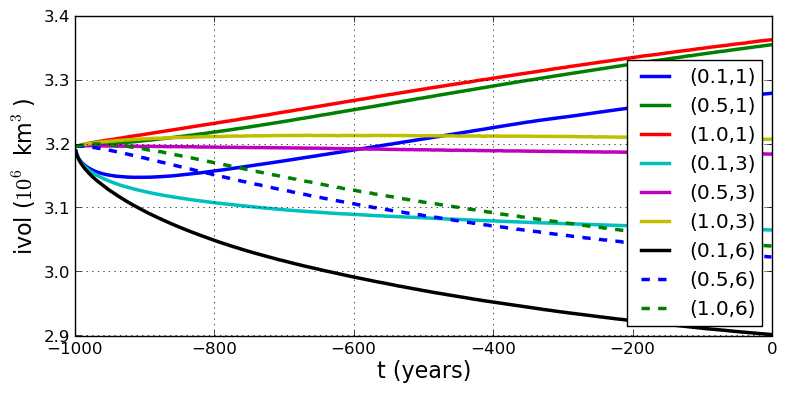
\includegraphics[width=4.5in,keepaspectratio=true]{ivol-param}

\caption{Time series of ice volume \texttt{ivol} from nine runs in our parameter study example, with parameter choices $(q,e)$ given.}
\label{fig:ivolparamstudy}
\end{figure}

We have not yet run PISM, but only asked one script to create nine others.  We now have the option of running them sequentially or in parallel.  Each script itself does a parallel run, over the \texttt{NN=4} processes specified by \texttt{param.sh} when generating the run scripts.  If you have $4 \times 9 = 36$ cores available then you can do the runs fully in parallel (this is \texttt{runparallel.sh} in \texttt{examples/std-greenland/}):
\begin{scriptvrb}
#!/bin/bash
for scriptname in $(ls p10km*sh) ; do
  echo ; echo "starting ${scriptname} ..."
  bash $scriptname &> out.$scriptname &  # start immediately in background
done
\end{scriptvrb}
%$
Otherwise you should do them in sequence (this is \texttt{runsequential.sh} in \texttt{examples/std-greenland/}):
\begin{scriptvrb}
#!/bin/bash
for scriptname in $(ls p10km*sh) ; do
  echo ; echo "starting ${scriptname} ..."
  bash $scriptname                       # will wait for completion
done
\end{scriptvrb}
%$
On the same old 2012-era 4 core laptop, \texttt{runsequential.sh} took a total of just under 7 hours to complete the whole parameter study.  The runs with $q=0.1$ (the more ``plastic'' end of the basal sliding spectrum) took up to four times longer than the $q=0.5$ and $q=1.0$ runs.  Roughly speaking, values of $q$ which are close to zero imply a subglacial till model with a true yield stress, and the result is that even small changes in overall ice sheet state (geometry, energy, \dots) will cause \emph{some} location to exceed its yield stress and suddenly change flow regime.  This will shorten the time steps.  By contrast, the $e$ value is much less significant in determining run times.

\begin{figure}[ht]
\centering
\mbox{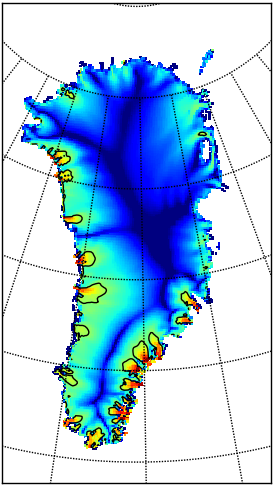
\includegraphics[height=2.5in,keepaspectratio=true]{p10km-01-1-csurf.png} 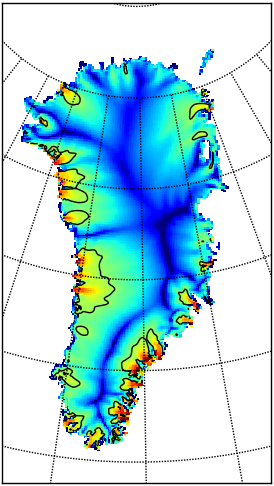
\includegraphics[height=2.5in,keepaspectratio=true]{p10km-01-3-csurf.png} 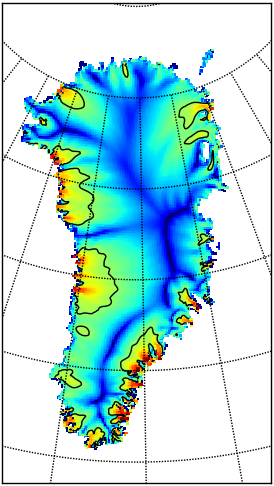
\includegraphics[height=2.5in,keepaspectratio=true]{p10km-01-6-csurf.png} \qquad \hspace{1.81in}}

\mbox{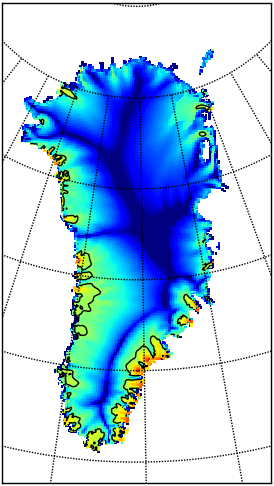
\includegraphics[height=2.5in,keepaspectratio=true]{p10km-05-1-csurf.png} 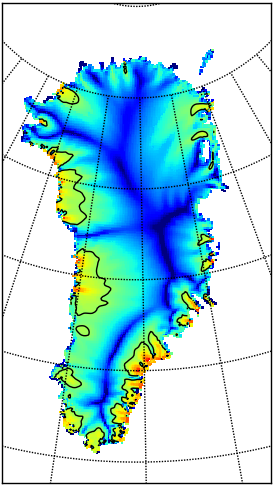
\includegraphics[height=2.5in,keepaspectratio=true]{p10km-05-3-csurf.png} 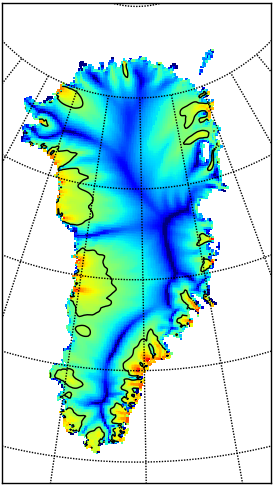
\includegraphics[height=2.5in,keepaspectratio=true]{p10km-05-6-csurf.png} 
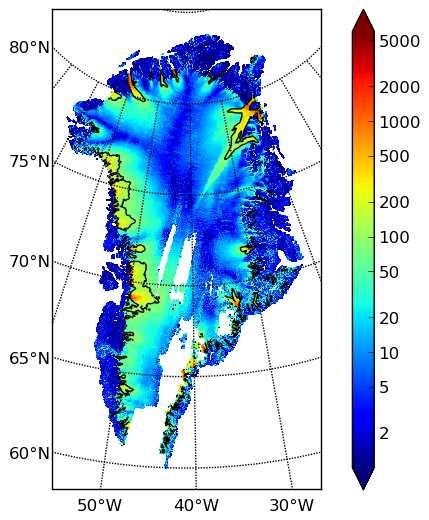
\includegraphics[height=2.5in,keepaspectratio=true]{Greenland-5km-v1p1-surfvelmag}}
\smallskip

\mbox{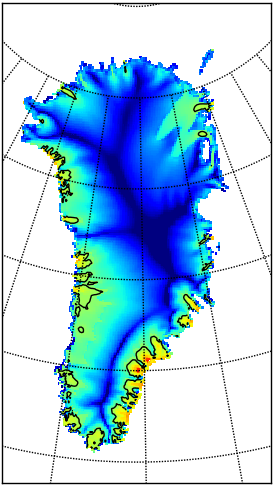
\includegraphics[height=2.5in,keepaspectratio=true]{p10km-1-1-csurf.png} 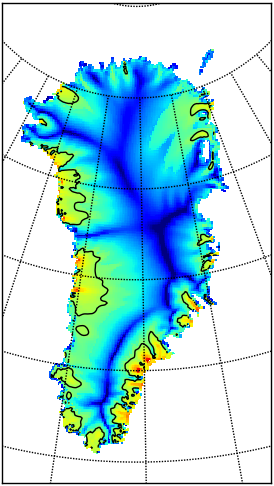
\includegraphics[height=2.5in,keepaspectratio=true]{p10km-1-3-csurf.png} 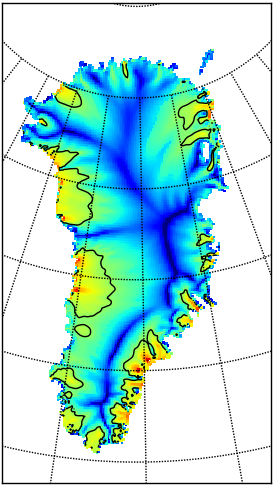
\includegraphics[height=2.5in,keepaspectratio=true]{p10km-1-6-csurf.png} \qquad \hspace{1.81in}}

\caption{Surface speed \texttt{velsurf_mag} from a 10\,km grid parameter study.  Right-most subfigure is observed data from \texttt{Greenland_5km_v1.1.nc}.  Top row: $q=0.1$ and $e=1,3,6$ (left-to-right).  Middle row: $q=0.5$.  Bottom row: $q=1.0$.  All subfigures have common color scale (velocity m/a), as shown in the right-most figure, with 100 m/a contour shown in all cases (solid black).}
\label{fig:paramstudy}
\end{figure}

On a supercomputer, the \texttt{runparallel.sh} script generally should be modified to submit jobs to the scheduler.  See example scripts \texttt{advanced/paramspawn.sh} and \texttt{advanced/paramsubmit.sh} for a parameter study that does this.  (But see your system administrator if you don't know what a ``job scheduler'' is!)  Of course, if you have a supercomputer then you can redo this parameter study on a 5\,km grid.

Results from these runs are seen in Figures \ref{fig:ivolparamstudy} and \ref{fig:paramstudy}.  In the former we see that the $(0.5,3)$ run simply continues the previous initialization run.  In some other graphs we see abrupt initial changes, caused by abrupt parameter change, e.g.~when the basal sliding becomes much more plastic ($q=0.1$).  In all cases with $e=1$ the flow slows and the sheet grows in volume as discharge decreases, while in all cases with $e=6$ the flow accelerates and the sheet shrinks in volume as discharge increases.

In Figure \ref{fig:paramstudy} we can compare the surface speed model results to observations.  Roughly speaking, the ice softness parameter $e$ has effects seen most-clearly by comparing the interior of the ice sheet; scan left-to-right for the $e=1,3,6$ subfigures.  The basal sliding exponent $q$ has effects seen most-clearly by comparing flow along the very steep margin, especially in the southern half of the ice sheet; scan top-to-bottom for $q=0.1,0.5,1.0$, going from nearly-plastic at top to linear at bottom.

From such figures we can make an informal assessment and comparison of the results, but objective assessment is important.  Example objective functionals include: \emph{(i)} compute the integral of the square (or other power) of the difference between the model and observed surface velocity \cite{AschwandenAdalgeirsdottirKhroulev}, or \emph{(ii)} compute the model-observed differences between the histogram of the number of cells with a given surface speed \cite{BKAJS}.  Note that these functionals are measuring the effects of changing a small number of parameters, namely two parameters in the current study.  So-called ``inversion'' might use the same objective functionals but with a much larger parameter space.  Inversion is therefore capable of achieving much smaller objective measures \cite{Habermannetal2013,Larouretal2012,Priceetal2011}, though at the cost of less understanding, perhaps, of the meaning of the optimal parameter values.

\clearpage  % does not lengthen pages, and puts Figure \ref{fig:paramstudy} before Table \ref{tab:NetCDFview}

\subsection{Handling NetCDF files}\label{subsect:nctoolsintro}  PISM takes one or more NetCDF files as input, then it does some computation, and then it produces one or more NetCDF files as output.  But other tools are usually needed to help to extract meaning from NetCDF files, and yet more NetCDF tools help with creating PISM input files or post-processing PISM output files.  Thus we finish this section with a list of NetCDF tools in Table \ref{tab:NetCDFview}.

The PISM authors use \texttt{ncview} and ``\texttt{ncdump -h}'' for quick visualization and metadata examination.  NCO has powerful command-line manipulation of NetCDF files, but requires some learning.  Another such command-line tool is CDO, but to use CDO on PISM files first run the script \texttt{nc2cdo.py}, from the \texttt{util/} PISM directory, on the file to fix the metadata so that CDO will understand the mapping.  Finally, Python scripts using the \texttt{netcdf4-python} package (see the PISM Installation Manual) are often the best way to non-trivially change a NetCDF file or make publishable figures from it.  Matlab also has good NetCDF I/O capabilities.

See Table \ref{tab:modelhierarchy} in subsection \ref{sec:model-hierarchy} for an overview on the data necessary for modeling.  For more information on the format of input files for PISM, see section \ref{sec:initboot}.

\newcommand{\netcdftool}[1]{#1\index{NetCDF!tools!#1}}
\begin{table}[ht]
\centering
\small
\begin{tabular}{llp{0.45\linewidth}}
  \toprule
  \textbf{Tool} & \textbf{Site} & \textbf{Function} \\
  \midrule
  & \url{www.unidata.ucar.edu/software/netcdf/} & root for NetCDF information \\
  \midrule
  \netcdftool{\texttt{ncdump}} & \emph{included with any NetCDF distribution} & dump binary NetCDF as \texttt{.cdl} (text) file \\
  \netcdftool{\texttt{ncgen}} & \emph{included with any NetCDF distribution} & convert \texttt{.cdl} file to binary NetCDF \\
  \midrule
  \netcdftool{CDO} & \url{http://code.zmaw.de/projects/cdo} & = Climate Data Operators; command-line tools, including conservative re-mapping \\
  \netcdftool{IDV} & \url{http://www.unidata.ucar.edu/software/idv/} & more complete visualization \\
  \netcdftool{NCO}\index{NCO (NetCDF Operators)} & \url{http://nco.sourceforge.net/} & = NetCDF Operators; command-line tools\\
  \netcdftool{NCL} &  \url{http://www.ncl.ucar.edu} & = NCAR Command Language\\
  \netcdftool{\texttt{ncview}} & \href{http://meteora.ucsd.edu/~pierce/ncview_home_page.html}{\texttt{meteora.ucsd.edu/$\sim$pierce}} & quick graphical view \\
  \netcdftool{PyNGL} &  \url{http://www.pyngl.ucar.edu} & Python version of NCL\\
  \bottomrule
\end{tabular}
\normalsize
\caption{A selection of tools for viewing and modifying NetCDF files.}
\label{tab:NetCDFview}
\end{table}


%%% Local Variables: 
%%% mode: latex
%%% TeX-master: "manual"
%%% End: 


% LocalWords:  metadata SPECMAP paleo html IDV
